\chapter{Fitting a Potential to a Spectrum}\label{ch:fitting}

\begin{chapterintro}
In Chapter~\ref{ch:finite-differences} you learned to run quantum mechanics forward: you are given a potential $V(x)$, you build a matrix, and a computer returns the energy levels. This chapter runs it backward. You are handed a list of target levels, and you must adjust a potential until its levels match the list. This is a \emph{fitting} problem, of the same family as drawing the best straight line through measured points, except that the ``line'' is a whole function $\delta V(x)$ and each ``point'' is an eigenvalue that depends on that function in a nonlinear way.

You already own every ingredient. First-order perturbation theory (Chapter~\ref{ch:perturbation}) tells you how much each level moves when you nudge the potential. Least squares and the singular value decomposition (Chapter~\ref{ch:least-squares}) tell you the best nudge to make when there are many levels and many knobs. The finite-difference solver (Chapter~\ref{ch:finite-differences}) tells you where the levels really are after the nudge. Put together and repeated, with a safety mechanism called damping, these become the Levenberg--Marquardt algorithm. We build it from scratch, then take apart, clause by clause, the exact recipe the paper uses. We also meet three ways of writing the correction $\delta V$ (cosines, Chebyshev polynomials and hat functions) and derive a rule of thumb, the \emph{coverage law}, that tells you how many basis functions are needed before a fit can reproduce essentially any list of levels.

Where this shows up in the paper: Sec.~II~C (``Hermitian fluctuation fit and out-of-sample protocol'', including the paragraph ``Other bases''), Appendix~A step~6 (the damping schedule), the first paragraph of Sec.~III (the coverage law and the in-sample numbers $0.186$ at $M=300$ and $<10^{-4}$ at $M=900$), and the in-sample columns of Tables~I, II and III. This chapter explains how the paper's fits are \emph{made}. Whether they \emph{predict} anything is a different question, taken up in Chapter~\ref{ch:generalization} and Chapter~\ref{ch:paper-memorization}.
\end{chapterintro}

\begin{prerequisites}
\item Chapter~\ref{ch:least-squares}: linear least squares, normal equations, the singular value decomposition (SVD), the pseudo-inverse and minimum-norm solutions, ridge regularization and filter factors.
\item Chapter~\ref{ch:perturbation}: the first-order energy shift $\delta E_n=\int|\psi_n|^2\,\delta V\,\dd x$, the sensitivity matrix $A_{nk}$, the second-order shift, and the condition that matrix elements be small compared with level spacings.
\item Chapter~\ref{ch:finite-differences}: the tridiagonal finite-difference Hamiltonian with Dirichlet walls, the discrete normalization $\sum_j\psi_j^2h=1$, Richardson extrapolation and bias-corrected targets $\tilde t_n$.
\item Chapter~\ref{ch:eigen}: symmetric matrices, real eigenvalues, positive definite matrices.
\item Chapter~\ref{ch:fourier-series}: the cosine basis $\cos(k\pi x/L)$ on $[-L,L]$ for even functions; beats.
\item Chapter~\ref{ch:asymptotics}: Newton's method for a single equation; Taylor's theorem with remainder.
\item Chapter~\ref{ch:bound-states}: eigenfunctions and levels of the infinite square well.
\item Chapter~\ref{ch:wkb}: the local wavenumber $\sqrt{E-V(x)}$, turning points and the WKB wavefunction (restated where used).
\item Chapter~\ref{ch:counting-zeros}: the smooth counting function $\Nsm$, the smooth zeros $s_n$ and the mean spacing $\gap_n$.
\item First-year physics: potential energy curves and classical turning points; standing waves on a string.
\end{prerequisites}

%==========================================================
\section{From levels to a potential: the inverse problem as least squares}\label{sec:fitting-problem}

\subsection{The forward map}

Throughout this chapter we use the units of the paper, $\hbar=2m=1$, so the Hamiltonian of a particle on a line is
\begin{equation}
H(c) \;=\; -\frac{\dd^2}{\dd x^2} + V(x) + \delta V(x;c),
\label{eq:fitting-H}
\end{equation}
where $V(x)$ is a fixed \emph{background} potential (in the paper, the Wu--Sprung potential of paper Eq.~(2), derived in Chapter~\ref{ch:wu-sprung}) and $\delta V$ is an adjustable \emph{correction}. We write the correction as a finite sum of chosen \emph{basis functions} $\phi_k(x)$:
\begin{equation}
\delta V(x;c) \;=\; \sum_{k=0}^{M-1} c_k\,\phi_k(x).
\label{eq:fitting-deltaV}
\end{equation}
Here $M$ is the number of basis functions (the \emph{basis size}), and the real numbers $c_0,c_1,\dots,c_{M-1}$ are the \emph{coefficients}, which we collect into a column vector $c$ with $M$ entries. The default basis in the paper is $\phi_k(x)=\cos(k\pi x/L)$, where $L$ is the half-width of the box $[-L,L]$ whose walls are at $x=\pm L$.

For each choice of $c$, the finite-difference solver of Chapter~\ref{ch:finite-differences} returns the energy levels $E_1(c)<E_2(c)<E_3(c)<\cdots$ of $H(c)$. The rule ``$c$ in, list of levels out'' is called the \emph{forward map}. We only ever need the lowest $n_{\rm fit}$ levels, where $n_{\rm fit}$ is the number of levels we try to match (the paper's $n_{\mathrm{fit}}$, for example 400).

\subsection{Targets, residuals and the objective}

The targets are numbers $\tilde t_1,\dots,\tilde t_{n_{\rm fit}}$ that we want the levels to equal. In the paper they are the bias-corrected zeros of Chapter~\ref{ch:finite-differences}: recall that $\tilde t_n=t_n+(E^{\rm grid}_n[\mathrm{smooth}]-E^{\rm Rich}_n[\mathrm{smooth}])$, where $t_n$ is the height of the $n$-th Riemann zero, $E^{\rm grid}_n[\mathrm{smooth}]$ is the $n$-th level of the uncorrected background on the working grid, and $E^{\rm Rich}_n[\mathrm{smooth}]$ is its Richardson extrapolant. For this chapter all that matters is that $\tilde t_n$ is a fixed list of numbers.

The \emph{residual} of level $n$ is the mismatch
\begin{equation}
r_n(c) \;=\; \tilde t_n - E_n(c), \qquad n=1,\dots,n_{\rm fit}.
\label{eq:fitting-residual}
\end{equation}
A positive residual means the level is too low and must be pushed up.

The paper quotes every error in units of the \emph{local mean spacing} $\gap_n$, the average distance between neighboring zeros near zero $n$. Recall (Chapter~\ref{ch:counting-zeros} derives it) that $\gap_n=2\pi/\log(s_n/2\pi)$, where $s_n$ is the $n$-th ``smooth zero'', the solution of $\Nsm(s_n)=n-\tfrac12$ with $\Nsm$ the smooth counting function of paper Eq.~(1). Dividing by $\gap_n$ makes errors at different heights comparable: an error of $0.1$ in energy is large where zeros are $1.3$ apart and small where they are $7.5$ apart. So we define the \emph{scaled residual}
\begin{equation}
\hat r_n(c) \;=\; \frac{r_n(c)}{\gap_n},
\label{eq:fitting-scaled}
\end{equation}
and the \emph{root mean square} (rms) error in mean spacings,
\begin{equation}
\mathrm{rms}(c) \;=\; \sqrt{\frac{1}{n_{\rm fit}}\sum_{n=1}^{n_{\rm fit}}\hat r_n(c)^2 }.
\label{eq:fitting-rms}
\end{equation}
The quantity we minimize is the \emph{objective}
\begin{equation}
\Phi(c) \;=\; \frac12\sum_{n=1}^{n_{\rm fit}}\hat r_n(c)^2 \;=\; \frac{n_{\rm fit}}{2}\,\mathrm{rms}(c)^2 .
\label{eq:fitting-Phi}
\end{equation}
The factor $\tfrac12$ is a convenience that removes a factor 2 from derivatives. Because $\mathrm{rms}=\sqrt{2\Phi/n_{\rm fit}}$ and the square root is an increasing function, any $c$ that lowers $\Phi$ lowers the rms, and the two have the same minimizers.

\begin{pitfall}
The paper's Appendix~A writes its update step in terms of ``$r$'', the residual vector, without saying whether each row has been divided by $\gap_n$. Dividing (\emph{weighting}) makes the least-squares step minimize exactly the quantity that is reported, the rms in mean spacings, so that is what we do in this chapter. The two choices need not give identical fits: $\gap_n$ falls from about $7.5$ at $n=1$ to about $1.3$ at $n=500$, so weighting changes how much the low levels count. The Zenodo scripts \cite{zenodo} settle what the paper's code does; our conclusions about the algorithm do not depend on it.
\end{pitfall}

\begin{sample}{Residuals and rms for three levels}
A trial potential gives the three lowest levels $E=(14.30,\,20.90,\,25.10)$. The targets are the first three zeros of RE1, $t=(14.134725,\,21.022040,\,25.010858)$, and the local mean spacings there are $\gap_1=7.500$, $\gap_2=5.279$, $\gap_3=4.486$ (computed from $\gap_n=2\pi/\log(s_n/2\pi)$). Find the residuals, the scaled residuals and the rms.

\emph{Step 1: residuals.} $r_n=t_n-E_n$: $r_1=14.134725-14.30=-0.165275$, $r_2=21.022040-20.90=0.122040$, $r_3=25.010858-25.10=-0.089142$.

\emph{Step 2: scaled residuals.} $\hat r_1=-0.165275/7.500=-0.02204$, $\hat r_2=0.122040/5.279=0.02312$, $\hat r_3=-0.089142/4.486=-0.01987$.

\emph{Step 3: squares and mean.} $\hat r_1^2=4.856\times10^{-4}$, $\hat r_2^2=5.344\times10^{-4}$, $\hat r_3^2=3.948\times10^{-4}$. Their mean is $(4.856+5.344+3.948)\times10^{-4}/3=4.716\times10^{-4}$.

\emph{Step 4: square root.}
\[
\boxed{\mathrm{rms}\approx 0.0217\ \text{mean spacings}}
\]
The levels are off by about two hundredths of a spacing, a very good fit in the paper's units.
\end{sample}

\subsection{Why the problem is nonlinear}

If each level moved in exact proportion to each coefficient, the residuals would be linear functions of $c$ and Chapter~\ref{ch:least-squares} would finish the job in one line. They are not. Recall from Chapter~\ref{ch:perturbation} that a small perturbation $\delta V$ shifts level $n$ by
\begin{equation}
\delta E_n \;=\; \int|\psi_n|^2\,\delta V\,\dd x \;+\; \sum_{m\neq n}\frac{\bigl|\langle m|\delta V|n\rangle\bigr|^2}{E_n-E_m} \;+\;\cdots,
\label{eq:fitting-pt}
\end{equation}
where $\psi_n$ is the normalized eigenfunction of level $n$ and $\langle m|\delta V|n\rangle=\int\psi_m\,\delta V\,\psi_n\,\dd x$. The first term is linear in $c$; the second is quadratic in $c$, because each matrix element is linear in $c$ and it appears squared. Doubling $c$ doubles the first term and quadruples the second. So $E_n(c)$ is a nonlinear function of $c$, and the inverse problem is a \emph{nonlinear least-squares problem}: minimize a sum of squares of functions that are not linear in the unknowns.

\begin{checkpoint}
You double every coefficient $c_k$ of a correction that already shifts level 7 by $+0.04$. Is the new shift exactly $+0.08$? Under what condition is it approximately $+0.08$?
\end{checkpoint}
\checkanswer{Not exactly: the second-order term of Eq.~\eqref{eq:fitting-pt} quadruples while the first-order term doubles. The new shift is close to $+0.08$ only if the second-order part is small, which by Chapter~\ref{ch:perturbation} requires the matrix elements $\langle m|\delta V|7\rangle$ to be small compared with the spacings $|E_7-E_m|$.}

\subsection{Which level is ``level $n$''?}

To compare $E_n$ with $\tilde t_n$ we match by index: the lowest level with the first target, and so on. This is unambiguous only if no two levels coincide, so that sorting by size is well defined and each level moves continuously as $c$ changes. For the matrices we use this is a theorem with a short proof.

The finite-difference Hamiltonian is a real symmetric tridiagonal $N\times N$ matrix with diagonal entries $d_j=2/h^2+V_j$ and off-diagonal entries $e=-1/h^2\neq 0$, where $h$ is the grid spacing. Suppose $v=(v_1,\dots,v_N)$ is an eigenvector with eigenvalue $E$. Row 1 of the eigen-equation reads $d_1v_1+e\,v_2=Ev_1$, so $v_2=(E-d_1)v_1/e$: $v_2$ is fixed by $v_1$. Row $j$ reads $e\,v_{j-1}+d_jv_j+e\,v_{j+1}=Ev_j$, so $v_{j+1}=[(E-d_j)v_j-e\,v_{j-1}]/e$: each component is fixed by the two before it. Hence every eigenvector with eigenvalue $E$ is $v_1$ times one fixed vector, namely the vector that the recursion generates when it is started from $v_1=1$. The value $v_1=0$ is not available to a genuine eigenvector: if $v_1=0$, row 1 gives $v_2=0$, then row 2 gives $v_3=0$, and so on, so $v=0$, which is not an eigenvector. A nonzero eigenvector therefore has $v_1\neq0$ and is a nonzero multiple of that one fixed vector. (The last row, $e\,v_{N-1}+d_Nv_N=Ev_N$, has no $v_{N+1}$ to solve for; it is a condition that only certain values of $E$ satisfy, and it adds no freedom.) So the eigenspace is one-dimensional. A real symmetric matrix has a full set of orthogonal eigenvectors (Chapter~\ref{ch:eigen}), so an eigenvalue of multiplicity two would need a two-dimensional eigenspace. Therefore all $N$ eigenvalues are distinct. (A similar argument for the differential equation itself, which we do not give here, shows that bound states of the continuum problem in one dimension are nondegenerate.)

\begin{keyideas}
\item The inverse problem: choose coefficients $c$ of $\delta V=\sum_kc_k\phi_k$ so that the levels $E_n(c)$ match targets $\tilde t_n$.
\item Residuals $r_n=\tilde t_n-E_n$, scaled by $\gap_n$; the objective $\Phi=\tfrac12\sum\hat r_n^2$ has the same minimizers as the rms in mean spacings.
\item $E_n(c)$ is nonlinear in $c$ (second-order perturbation theory), so this is a nonlinear least-squares problem.
\item Levels of the tridiagonal Hamiltonian are never degenerate, so matching level $n$ to target $n$ by sorting is well defined.
\end{keyideas}

%==========================================================
\section{Linearization: the sensitivity matrix}\label{sec:fitting-sensitivity}

\subsection{Derivative of a level with respect to a coefficient}

Every method in this chapter rests on one question: if we change $c$ by a small amount $\delta c$, how do the levels move? Suppose the current coefficients are $c$, and let $E_n$ and $\psi_n$ be the eigenvalues and normalized eigenfunctions of $H(c)$. Changing $c$ to $c+\delta c$ changes the Hamiltonian by
\[
H(c+\delta c)-H(c)=\sum_k(c_k+\delta c_k)\phi_k-\sum_kc_k\phi_k=\sum_{k=0}^{M-1}\delta c_k\,\phi_k(x).
\]
This is a perturbing potential added to $H(c)$. First-order perturbation theory (Chapter~\ref{ch:perturbation}), applied with $H(c)$ as the unperturbed operator, gives
\begin{align}
E_n(c+\delta c) &= E_n(c)+\int|\psi_n(x)|^2\sum_k\delta c_k\,\phi_k(x)\,\dd x+\order(\norm{\delta c}^2) \nonumber\\
&= E_n(c)+\sum_k\delta c_k\int|\psi_n(x)|^2\phi_k(x)\,\dd x+\order(\norm{\delta c}^2)\quad\text{(integral of a sum)}\nonumber\\
&= E_n(c)+\sum_kA_{nk}(c)\,\delta c_k+\order(\norm{\delta c}^2),
\label{eq:fitting-lin}
\end{align}
with the \emph{sensitivity matrix}
\begin{equation}
A_{nk}(c) \;=\; \int_{-L}^{L}|\psi_n(x;c)|^2\,\phi_k(x)\,\dd x .
\label{eq:fitting-A}
\end{equation}
Here $\norm{\delta c}$ is the length of the vector $\delta c$ and $\order(\norm{\delta c}^2)$ collects terms at least quadratic in $\delta c$ (the second-order term of Eq.~\eqref{eq:fitting-pt} and beyond). Comparing Eq.~\eqref{eq:fitting-lin} with the definition of a partial derivative,
\[
\frac{\partial E_n}{\partial c_k} \;=\; A_{nk}(c).
\]
In words: the rate at which level $n$ moves when you turn knob $k$ is the overlap of the knob's shape $\phi_k$ with the probability density $|\psi_n|^2$ of the current state. This is often called the Hellmann--Feynman relation. In general form: if a Hamiltonian depends on a parameter $\alpha$, a nondegenerate level obeys $\dd E_n/\dd\alpha=\langle\psi_n|\partial H/\partial\alpha|\psi_n\rangle$. This is nothing but first-order perturbation theory (Chapter~\ref{ch:perturbation}) applied to the small change $(\partial H/\partial\alpha)\,\delta\alpha$ of the Hamiltonian, divided by $\delta\alpha$. Here $\alpha=c_k$, and by Eqs.~\eqref{eq:fitting-H} and \eqref{eq:fitting-deltaV}, $\partial H/\partial c_k=\phi_k(x)$. Note that $A$ depends on $c$, because the eigenfunctions $\psi_n$ do.

The $n_{\rm fit}\times M$ matrix $A$ is the \emph{Jacobian} of the forward map (the matrix of all first partial derivatives). From Eq.~\eqref{eq:fitting-residual}, residuals move the opposite way to levels:
\begin{equation}
r(c+\delta c)\;\approx\;r(c)-A(c)\,\delta c, \qquad \hat r(c+\delta c)\;\approx\;\hat r(c)-\hat A(c)\,\delta c,
\label{eq:fitting-rlin}
\end{equation}
where $\hat A_{nk}=A_{nk}/\gap_n$ is the sensitivity matrix with row $n$ divided by the same spacing as residual $n$.

\begin{beyond}
We take on trust that each nondegenerate eigenvalue $E_n(c)$ is a differentiable (indeed smooth) function of $c$, so that the remainder in Eq.~\eqref{eq:fitting-lin} really is of order $\norm{\delta c}^2$. For finite matrices with distinct eigenvalues, which we proved in Section~\ref{sec:fitting-problem}, this follows from the implicit function theorem applied to the characteristic polynomial; texts on the perturbation theory of linear operators give the full proof. Chapter~\ref{ch:perturbation} already gave the first and second terms of the expansion explicitly.
\end{beyond}

\subsection{The constant mode}

If one basis function is the constant $\phi_0(x)=1$ (true for the cosine basis with $k=0$), then
\[
A_{n0}=\int|\psi_n|^2\cdot1\,\dd x=1\qquad\text{for every }n,
\]
because each $\psi_n$ is normalized. A constant added to the potential shifts every level by the same amount. In fact, $H+c_0$ has exactly the same eigenvectors as $H$ with every eigenvalue raised by exactly $c_0$, so this one knob acts linearly to all orders.

\subsection{The discrete version and a normalization trap}

On a grid of $N$ interior points $x_j=-L+jh$, $h=2L/(N+1)$, the integral in Eq.~\eqref{eq:fitting-A} becomes a sum, $A_{nk}=\sum_j|\psi_n(x_j)|^2\phi_k(x_j)\,h$, with the grid normalization $\sum_j|\psi_n(x_j)|^2h=1$ of Chapter~\ref{ch:finite-differences} (paper Appendix~A step~9). A numerical eigensolver, however, returns eigenvectors $w_n$ of unit \emph{Euclidean} length, $\sum_jw_{jn}^2=1$. (We write $w$, not $v$, for these eigenvectors, because $v_i$ will denote singular vectors in Section~\ref{sec:fitting-svd}.) The two are related by $\psi_n(x_j)=w_{jn}/\sqrt h$, so
\begin{equation}
A_{nk}=\sum_j\frac{w_{jn}^2}{h}\,\phi_k(x_j)\,h=\sum_jw_{jn}^2\,\phi_k(x_j).
\label{eq:fitting-Adisc}
\end{equation}
The factors of $h$ cancel.

\begin{pitfall}
If you rescale the solver's vectors to $\psi=w/\sqrt h$ and then forget the factor $h$ in the sum, every entry of $A$ comes out too large by $1/h$, which on the paper's working grid ($N=6000$, $L=44.883$, so $1/h\approx67$) is a factor of about 67. Gauss--Newton steps would then be 67 times too small. A one-line test catches this: with $\phi_0=1$, every $A_{n0}$ must equal 1.
\end{pitfall}

\begin{sample}{The sensitivity matrix of the box}
Take RE3, the infinite square well on $[-L,L]$ ($V=0$, Dirichlet walls), with the cosine basis $\phi_k=\cos(k\pi x/L)$. Compute $A_{nk}$ exactly.

\emph{Step 1: eigenfunctions.} From Chapter~\ref{ch:bound-states}, $\psi_n(x)=\frac{1}{\sqrt L}\sin\!\left(\frac{n\pi(x+L)}{2L}\right)$, $n=1,2,\dots$, with $E_n=(n\pi/2L)^2$.

\emph{Step 2: the density.} Using $\sin^2\alpha=\tfrac12(1-\cos2\alpha)$,
\[
|\psi_n|^2=\frac{1}{2L}\left[1-\cos\!\left(\frac{n\pi(x+L)}{L}\right)\right].
\]
Since $\cos(\theta+n\pi)=(-1)^n\cos\theta$, the bracket is $1-(-1)^n\cos(n\pi x/L)$, so
\[
|\psi_n|^2=\frac{1}{2L}\left[1-(-1)^n\cos\frac{n\pi x}{L}\right].
\]

\emph{Step 3: overlaps.} For $k=0$: $A_{n0}=\frac{1}{2L}\bigl[2L-(-1)^n\int_{-L}^L\cos\frac{n\pi x}{L}\dd x\bigr]=\frac{1}{2L}[2L-0]=1$. For $k\ge1$: $\int_{-L}^L\cos\frac{k\pi x}{L}\dd x=0$, and by the orthogonality of Chapter~\ref{ch:fourier-series}, $\int_{-L}^L\cos\frac{n\pi x}{L}\cos\frac{k\pi x}{L}\dd x=L\,\delta_{nk}$ for $n,k\ge1$, where $\delta_{nk}$ is 1 if $n=k$ and 0 otherwise. So $A_{nk}=\frac{1}{2L}\bigl[0-(-1)^nL\,\delta_{nk}\bigr]$.

\emph{Step 4: result.}
\[
\boxed{A_{n0}=1,\qquad A_{nk}=\frac{(-1)^{n+1}}{2}\,\delta_{nk}\quad(k\ge1)}
\]
To first order, cosine $k$ moves only level $n=k$ (up by $c_k/2$ for odd $n$, down for even $n$), and $c_0$ moves all levels together. For the finite-difference box with $N$ interior grid points the same values hold exactly, provided $n+k<N+1$ (Problem~8); on fine grids this covers every $n$ and $k$ of interest.
\end{sample}

The physical reason for the result is worth remembering. The density $|\psi_n|^2$ is a constant plus a ripple $\cos(n\pi x/L)$, a standing wave with $n$ humps across the box. A cosine perturbation can push on level $n$ only if it has the same ripple, like pushing a child on a swing in time with the swing. In the box, the wavenumber of the ripple of level $n$ is $n\pi/L=2\sqrt{E_n}$. Keep that factor of 2 in mind: it returns in Section~\ref{sec:fitting-coverage}.

\begin{sample}{One linearized step in the box}
In the box of RE3 with $M=4$ cosines ($k=0,1,2,3$), we want first-order shifts $d=(0.01,\,-0.02,\,0.03)$ of levels 1, 2, 3. Find the coefficient vector of smallest length that produces them.

\emph{Step 1: equations.} By the Sample Problem ``The sensitivity matrix of the box'', $\delta E_n=c_0+\tfrac12(-1)^{n+1}c_n$, so
\[
c_0+\tfrac12c_1=0.01,\qquad c_0-\tfrac12c_2=-0.02,\qquad c_0+\tfrac12c_3=0.03 .
\]
Three equations, four unknowns: the system is underdetermined (Chapter~\ref{ch:least-squares}) and has infinitely many solutions.

\emph{Step 2: express in terms of $c_0$.} Writing $\epsilon_n=(-1)^{n+1}$, the equations give $c_n=2\epsilon_n(d_n-c_0)$, so $c_n^2=4(d_n-c_0)^2$.

\emph{Step 3: minimize the length.} $\norm c^2=c_0^2+4\sum_{n=1}^3(d_n-c_0)^2$. Setting the derivative with respect to $c_0$ to zero:
\[
2c_0-8\sum_n(d_n-c_0)=0\;\Rightarrow\;2c_0-8\sum_nd_n+24c_0=0\;\Rightarrow\;c_0=\frac{4}{13}\sum_nd_n=\frac{4\times0.02}{13}.
\]

\emph{Step 4: numbers.} $c_0=0.0061538$, $c_1=2(0.01-0.0061538)=0.0076923$, $c_2=-2(-0.02-0.0061538)=0.0523077$, $c_3=2(0.03-0.0061538)=0.0476923$.
\[
\boxed{c\approx(0.00615,\;0.00769,\;0.05231,\;0.04769)}
\]
This is exactly what the pseudo-inverse of Chapter~\ref{ch:least-squares} returns (you can confirm it with \texttt{numpy.linalg.pinv}).
\end{sample}

\begin{pitfall}
Do not expect the step of the Sample Problem ``One linearized step in the box'' to produce the shifts it was designed for. In the box with $L=44.883$, the lowest levels are extremely close together: $E_2-E_1=3\pi^2/(4L^2)\approx0.00367$ and $E_3-E_1=2\pi^2/L^2\approx0.00980$. The off-diagonal matrix elements are as large as the diagonal ones. For example, with $\theta=\pi(x+L)/(2L)$, $\psi_1\psi_3=\frac{1}{2L}(\cos2\theta-\cos4\theta)$ and $\cos(2\pi x/L)=\cos4\theta$, so
\[
\langle1|\cos\tfrac{2\pi x}{L}|3\rangle=\frac{1}{2L}\cdot\frac{2L}{\pi}\int_0^\pi(\cos2\theta-\cos4\theta)\cos4\theta\,\dd\theta=\frac{1}{\pi}\left(0-\frac{\pi}{2}\right)=-\frac12 .
\]
The second-order term this coupling contributes to level 1 is of size $(c_2/2)^2/(E_3-E_1)\approx(0.026)^2/0.0098\approx0.07$, seven times the first-order shift of $0.01$ we aimed for. The validity condition of Chapter~\ref{ch:perturbation} fails badly. The cure is to take a linearized step, recompute the true levels, and repeat, with steps short enough that each one is trustworthy. That is the subject of the next three sections.
\end{pitfall}

\subsection{The sensitivity matrix of the Wu--Sprung well}

\Cref{fig:fitting-sensitivity} compares $|A_{nk}|$ for the box (left) and for the Wu--Sprung potential in the same box (right). In the box the only nonzero entries with $k\ge1$ lie on the diagonal $k=n$. In the Wu--Sprung well each level responds to a whole range of cosines, and the range widens as $n$ grows. Even for the lowest level the range is not small: the cutoff introduced below sits at $k=2L\sqrt{E_1-V_0}/\pi\approx60$ if we take $E_1\approx t_1=14.13$, because the lowest level lies about $4.4$ above the bottom of the well. The dashed curves mark $k=2L\sqrt{E_n-V_{\min}}/\pi$, with $V_{\min}$ the bottom of the well ($0$ for the box, $V_0=3.10073\pi\approx9.7412$ for Wu--Sprung). Above the curve the entries fall off sharply. Section~\ref{sec:fitting-coverage} explains why.

\begin{figure}[htbp]\centering
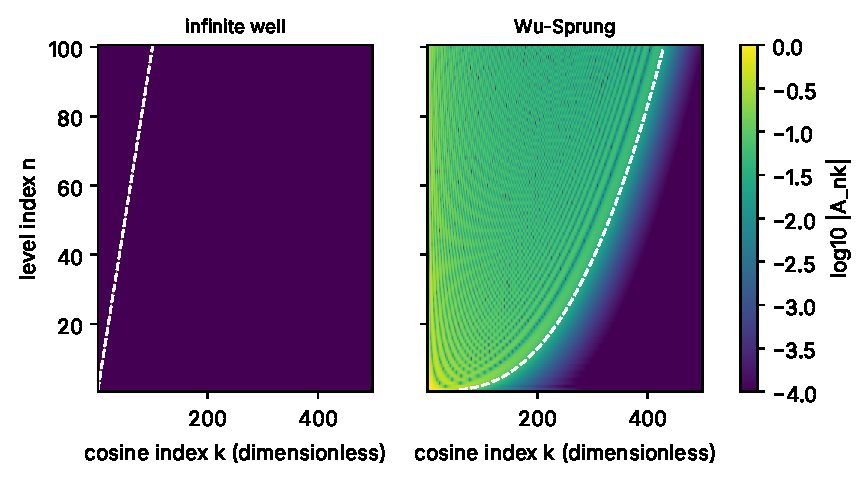
\includegraphics[width=0.95\linewidth]{figs/fitting_sensitivity.pdf}
\caption{Magnitude of the first-order sensitivity matrix $A_{nk}=\int|\psi_n|^2\cos(k\pi x/L)\,\dd x$ (color, $\log_{10}$ scale, entries below $10^{-4}$ shown dark) for the lowest 100 levels and $k=1,\dots,499$, in a box of half-width $L=44.883$ (units $\hbar=2m=1$). Left: infinite well, where only $k=n$ responds. Right: the Wu--Sprung potential, where level $n$ responds to all $k$ up to roughly the dashed curve $k=2L\sqrt{E_n-V_0}/\pi$ and very weakly beyond it.}
\label{fig:fitting-sensitivity}
\end{figure}

\begin{checkpoint}
For the Wu--Sprung potential with the cosine basis, what is $A_{37,0}$? What would it be for a hat basis if you summed $A_{37,j}$ over all hats $j$?
\end{checkpoint}
\checkanswer{$A_{37,0}=\int|\psi_{37}|^2\dd x=1$ by normalization. For hats, $\sum_j\phi_j(x)=1$ at every $x$ (Section~\ref{sec:fitting-bases}), so $\sum_jA_{37,j}=\int|\psi_{37}|^2\sum_j\phi_j\,\dd x=1$ as well.}

\begin{keyideas}
\item $\partial E_n/\partial c_k=A_{nk}=\int|\psi_n|^2\phi_k\,\dd x$, evaluated with the \emph{current} eigenfunctions; $A$ is the Jacobian of the forward map.
\item Residuals linearize as $r(c+\delta c)\approx r(c)-A\,\delta c$ (Eq.~\eqref{eq:fitting-rlin}).
\item With solver eigenvectors $w_n$ of unit Euclidean norm, $A_{nk}=\sum_jw_{jn}^2\phi_k(x_j)$; test with $A_{n0}=1$.
\item In the box, cosine $k$ moves only level $k$ to first order; in the Wu--Sprung well each level responds to many cosines.
\item Linearized steps can be badly wrong when level spacings are small, so steps must be iterated and controlled.
\end{keyideas}

%==========================================================
\section{Gauss--Newton: iterate the linear fit}\label{sec:fitting-gn}
% DYK-BEGIN
\begin{didyouknow}{One Spectrum Is Not Enough}
In 1946 G\"oran Borg proved that one list of energy levels does not in general determine a one-dimensional potential, but two spectra with different boundary conditions do. There is an important exception: if the potential is known to be symmetric, one spectrum suffices. Israel Gel'fand and Boris Levitan gave a constructive inversion method in 1951. Fitting a potential to levels is an old inverse problem.
\end{didyouknow}
% DYK-END

\subsection{The idea}

At the current $c$, the linearization Eq.~\eqref{eq:fitting-rlin} turns the nonlinear problem into a linear one: choose $\delta c$ to minimize
\[
\frac12\norm{\hat r-\hat A\,\delta c}^2 .
\]
This is exactly the linear least-squares problem of Chapter~\ref{ch:least-squares}, with $\hat A$ as the design matrix and $\hat r$ as the data. Its solution satisfies the normal equations
\begin{equation}
\hat A^\top\hat A\,\delta c \;=\; \hat A^\top\hat r .
\label{eq:fitting-gn}
\end{equation}
Taking that step, recomputing the true levels at $c+\delta c$, and repeating, is the \emph{Gauss--Newton method}:

\begin{enumerate}
\item Start from $c^{(0)}$ (the paper starts from $c=0$).
\item At $c^{(i)}$: solve the eigenproblem for $E_n$ and $\psi_n$; form $\hat r$ and $\hat A$.
\item Solve Eq.~\eqref{eq:fitting-gn} for $\delta c$.
\item Set $c^{(i+1)}=c^{(i)}+\delta c$ and return to step 2.
\end{enumerate}

With one level and one coefficient, Eq.~\eqref{eq:fitting-gn} reads $J^2\delta c=Jr$ with $J=\partial E/\partial c$, so $\delta c=r/J$. That is Newton's method (Chapter~\ref{ch:asymptotics}) for solving $E(c)=\tilde t$. Gauss--Newton is the many-equation, least-squares generalization of Newton's method.

If the levels happen to depend linearly on $c$ (for instance, a constant shift $c_0$ only), the linearization is exact and one Gauss--Newton step lands on the minimum.

\subsection{A two-level model you can do by hand}

We need a nonlinear example small enough to iterate on paper. Take the $2\times2$ real symmetric Hamiltonian
\[
H(c)=\begin{pmatrix}1&c\\ c&3\end{pmatrix}.
\]
Its characteristic polynomial (Chapter~\ref{ch:eigen}) is $(1-E)(3-E)-c^2=E^2-4E+3-c^2=0$, so
\[
E_\pm(c)=2\pm\sqrt{4-3+c^2}=2\pm\sqrt{1+c^2}.
\]
We fit the single coefficient $c$ so that the lower level equals the target $0.5$. Exact answer: $2-\sqrt{1+c^2}=0.5\Rightarrow\sqrt{1+c^2}=1.5\Rightarrow c^2=1.25$, so $c_*=\pm1.118034$.

The derivative is $J(c)=\dd E_-/\dd c=-c/\sqrt{1+c^2}$. Hellmann--Feynman gives the same thing: $\partial H/\partial c=\begin{pmatrix}0&1\\1&0\end{pmatrix}$, so $J=\langle\psi|\partial H/\partial c|\psi\rangle=2\psi_1\psi_2$ for the normalized lower eigenvector $(\psi_1,\psi_2)$.

\begin{sample}{Gauss--Newton on the two-level model}
Starting from $c^{(0)}=0.5$, take three Gauss--Newton steps toward $E_-(c)=0.5$.

\emph{Step 1: at $c^{(0)}=0.5$.} $\sqrt{1.25}=1.118034$, so $E_-=0.881966$, $r=0.5-0.881966=-0.381966$, $J=-0.5/1.118034=-0.447214$. As a check, the lower eigenvector satisfies $(1-E)\psi_1+c\psi_2=0$, so $\psi_2/\psi_1=(E-1)/c=-0.236068$; normalizing gives $(\psi_1,\psi_2)=(0.973249,\,-0.229753)$ and $2\psi_1\psi_2=-0.447214=J$.

\emph{Step 2: first step.} $\delta c=r/J=0.854102$, so $c^{(1)}=1.354102$. There $\sqrt{1+c^2}=1.683328$, $E_-=0.316672$: we overshot.

\emph{Step 3: second step.} $r=0.183328$, $J=-1.354102/1.683328=-0.804419$, $\delta c=-0.227901$, so $c^{(2)}=1.126201$.

\emph{Step 4: third step.} At $c^{(2)}$: $E_-=0.493903$, $r=0.006097$, $J=-0.747761$, $\delta c=-0.008153$, so $c^{(3)}=1.118047$.

\[
\boxed{c^{(1)}=1.3541,\quad c^{(2)}=1.1262,\quad c^{(3)}=1.11805\ \ (c_*=1.118034)}
\]
The errors $c^{(i)}-c_*$ are $-0.618$, $0.236$, $0.0082$, $0.000013$: once close, each error is roughly a constant times the square of the previous one. The error analysis of Newton's method predicts the constant; here is the argument. Write $f(c)=E_-(c)-0.5$. Since $r=-f$ and $J=f'$, the Gauss--Newton step is $c_{i+1}=c_i-f(c_i)/f'(c_i)$. Taylor's theorem about $c_i$ gives, for some $\xi$ between $c_i$ and $c_*$,
\[
0=f(c_*)=f(c_i)+f'(c_i)(c_*-c_i)+\tfrac12f''(\xi)(c_*-c_i)^2 .
\]
Dividing by $f'(c_i)$ and moving terms,
\[
c_i-\frac{f(c_i)}{f'(c_i)}-c_*=\frac{f''(\xi)}{2f'(c_i)}(c_i-c_*)^2 .
\]
The left side is $c_{i+1}-c_*=e_{i+1}$, with $e_i=c_i-c_*$. Close to the solution $f'(c_i)\approx f'(c_*)$ and $f''(\xi)\approx f''(c_*)$; also $f'=E_-'$ and $f''=E_-''$. Hence $e_{i+1}\approx\bigl[E_-''(c_*)/2E_-'(c_*)\bigr]\,e_i^2$, with constant of size $\abs{E_-''(c_*)/2E_-'(c_*)}$. Here $E_-'(c)=-c(1+c^2)^{-1/2}$, and differentiating once more,
\[
E_-''(c)=-(1+c^2)^{-1/2}+c^2(1+c^2)^{-3/2}=-(1+c^2)^{-3/2}.
\]
At $c_*$, $1+c_*^2=2.25$, so $E_-'(c_*)=-1.118034/1.5=-0.7454$ and $E_-''(c_*)=-1/1.5^3=-0.2963$, giving the constant $0.2963/(2\times0.7454)=0.199$. Indeed $0.199\times0.0082^2=1.3\times10^{-5}$, the last error. The first two errors are too large for this asymptotic rule to apply. Quadratic convergence of this kind is typical of Newton-type methods when the fit can be made exact. But the first step overshot by a lot.
\end{sample}

\Cref{fig:fitting-landscape} shows the landscape. The absolute residual $|r(c)|$ (equivalently the objective $\Phi=\tfrac12r^2$) has two equally good minima at $c=\pm1.118$ and a local \emph{maximum} at $c=0$.

\begin{figure}[htbp]\centering
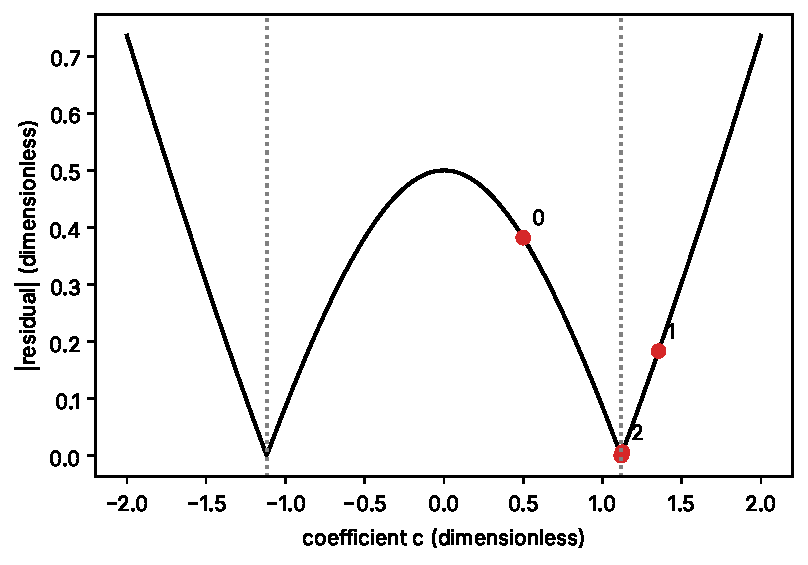
\includegraphics[width=0.85\linewidth]{figs/fitting_landscape.pdf}
\caption{The two-level model $H=\begin{pmatrix}1&c\\c&3\end{pmatrix}$ fitted so that its lower eigenvalue equals $0.5$. Curve: absolute residual $|0.5-E_-(c)|$ (dimensionless). Dots: Gauss--Newton iterates from $c=0.5$ (Sample Problem ``Gauss--Newton on the two-level model''), which overshoot once and then converge rapidly. The two minima at $c=\pm\sqrt{1.25}$ fit equally well; at $c=0$ the slope vanishes and a Gauss--Newton step is undefined.}
\label{fig:fitting-landscape}
\end{figure}

\subsection{How Gauss--Newton fails}

The two-level model already displays the three failure modes that matter for the paper's problem.

\emph{Zero sensitivity.} At $c=0$, $J=0$ and $\delta c=r/J$ is undefined. In the many-parameter case the analogue is a matrix $\hat A^\top\hat A$ with zero or tiny eigenvalues, so Eq.~\eqref{eq:fitting-gn} has no unique solution or an enormous one.

\emph{Overshoot.} Far from the solution the linear model is poor and a full step can land somewhere worse, or (in harder problems) diverge. The pitfall at the end of Section~\ref{sec:fitting-sensitivity} showed that the Wu--Sprung problem, with its many closely spaced levels, is prone to this.

\emph{Too many knobs.} When $M>n_{\rm fit}$ the $M\times M$ matrix $\hat A^\top\hat A$ has rank at most $n_{\rm fit}<M$ (Chapter~\ref{ch:least-squares}), so it is singular and Eq.~\eqref{eq:fitting-gn} has infinitely many solutions. The paper's fits include such cases, for instance $M=900$ on 500 levels (Sec.~III), $M=400$ on 200 odd-indexed levels (Table~III), and $M=400$ on zeros 1--300 (Table~I).

All three are cured by one modification, which we now derive.

\begin{checkpoint}
Your fit has a single knob, a constant shift $c_0$ with $\phi_0=1$. How many Gauss--Newton steps does it need, and what is the answer?
\end{checkpoint}
\checkanswer{One step: the levels depend linearly on $c_0$ with $A_{n0}=1$, so the linearization is exact. Unweighted, the normal equation gives $n_{\rm fit}\,c_0=\sum_nr_n$, the mean residual; with weights it is the weighted mean $\sum_nr_n/\gap_n^2\big/\sum_n1/\gap_n^2$.}

\begin{keyideas}
\item Gauss--Newton: at each iterate solve the linear least-squares problem $\min\norm{\hat r-\hat A\delta c}$, via $\hat A^\top\hat A\,\delta c=\hat A^\top\hat r$, then recompute.
\item It is the least-squares version of Newton's method; fast near a solution.
\item It fails with zero or tiny sensitivities, overshoots far from the solution, and its step is not unique when $M>n_{\rm fit}$.
\end{keyideas}

%==========================================================
\section{Gradient descent and the Levenberg--Marquardt compromise}\label{sec:fitting-lm}

\subsection{The downhill direction}

A completely different way to lower $\Phi$ is to walk downhill. The gradient $\nabla\Phi$ is the vector of partial derivatives $\partial\Phi/\partial c_k$. From Eq.~\eqref{eq:fitting-Phi} and the chain rule,
\begin{align*}
\frac{\partial\Phi}{\partial c_k}&=\sum_n\hat r_n\frac{\partial\hat r_n}{\partial c_k}\\
&=\sum_n\hat r_n\left(-\frac{1}{\gap_n}\frac{\partial E_n}{\partial c_k}\right)\quad\text{(Eq.~\eqref{eq:fitting-scaled}, $\tilde t_n$ fixed)}\\
&=-\sum_n\hat r_n\hat A_{nk},
\end{align*}
that is,
\begin{equation}
\nabla\Phi=-\hat A^\top\hat r .
\label{eq:fitting-grad}
\end{equation}
\emph{Steepest descent} takes $\delta c=\eta\,\hat A^\top\hat r$ with a small positive step size $\eta$. To first order the change in $\Phi$ is $\nabla\Phi\cdot\delta c=-\eta\norm{\hat A^\top\hat r}^2<0$, so a small enough step always goes downhill (unless the gradient is already zero). The price is speed: in a long narrow valley the gradient points mostly across the valley, and the walker zigzags.

\subsection{Damped least squares}

Gauss--Newton is fast but reckless; steepest descent is safe but slow. In 1963 Marquardt \cite{marquardt}, building on earlier work of Levenberg, proposed a single formula that slides between them. Keep the linear model, but add a penalty for long steps:
\begin{equation}
Q(\delta c)=\frac12\norm{\hat r-\hat A\,\delta c}^2+\frac12\lambda'\norm{\delta c}^2,\qquad\lambda'>0 .
\label{eq:fitting-Q}
\end{equation}
The \emph{damping parameter} $\lambda'$ sets how strongly long steps are penalized. To minimize $Q$, write it out in components, $Q=\tfrac12\sum_n(\hat r_n-\sum_l\hat A_{nl}\delta c_l)^2+\tfrac12\lambda'\sum_l\delta c_l^2$, and set each partial derivative to zero:
\begin{align*}
\frac{\partial Q}{\partial\delta c_k}&=\sum_n\Bigl(\hat r_n-\sum_l\hat A_{nl}\delta c_l\Bigr)(-\hat A_{nk})+\lambda'\delta c_k=0\\
&\Rightarrow\;\sum_l\Bigl(\sum_n\hat A_{nk}\hat A_{nl}\Bigr)\delta c_l+\lambda'\delta c_k=\sum_n\hat A_{nk}\hat r_n .
\end{align*}
In matrix form,
\begin{equation}
\bigl(\hat A^\top\hat A+\lambda'I\bigr)\,\delta c=\hat A^\top\hat r ,
\label{eq:fitting-lm}
\end{equation}
with $I$ the $M\times M$ identity. This is the \emph{Levenberg--Marquardt} (LM) step. Notice its family resemblance to ridge regression (Chapter~\ref{ch:least-squares}): the same $+\lambda' I$, but penalizing the \emph{step} $\delta c$, not the coefficients $c$.

The matrix $B=\hat A^\top\hat A+\lambda'I$ is always invertible for $\lambda'>0$. For any nonzero vector $z$, $z^\top Bz=z^\top\hat A^\top\hat Az+\lambda'z^\top z=\norm{\hat Az}^2+\lambda'\norm z^2>0$, so $B$ is symmetric and positive definite, its eigenvalues are all positive (Chapter~\ref{ch:eigen}), and it has an inverse. So the LM step exists even when $M>n_{\rm fit}$ or when sensitivities vanish.

\subsection{The two limits}

\emph{Small damping.} As $\lambda'\to0$, Eq.~\eqref{eq:fitting-lm} becomes the Gauss--Newton equation~\eqref{eq:fitting-gn}.

\emph{Large damping.} Factor out $\lambda'$: $B=\lambda'(I+\hat A^\top\hat A/\lambda')$. When $\lambda'$ is much larger than every eigenvalue of $\hat A^\top\hat A$, the second term is small and $B^{-1}\approx I/\lambda'$, so
\[
\delta c\approx\frac{1}{\lambda'}\hat A^\top\hat r ,
\]
which by Eq.~\eqref{eq:fitting-grad} is steepest descent with step size $\eta=1/\lambda'$. What is neglected is the term $\hat A^\top\hat A/\lambda'$, of relative size $\sigma_1^2/\lambda'$ where $\sigma_1^2$ is the largest eigenvalue of $\hat A^\top\hat A$.

\subsection{Every LM step points downhill}

At first order the change in $\Phi$ along the LM step is
\[
\nabla\Phi\cdot\delta c=-(\hat A^\top\hat r)^\top B^{-1}(\hat A^\top\hat r).
\]
$B^{-1}$ is positive definite (its eigenvalues are the reciprocals of those of $B$), so this is negative whenever $\hat A^\top\hat r\neq0$. Moreover, as $\lambda'$ grows the step shrinks like $1/\lambda'$, its first-order decrease $\approx\norm{\hat A^\top\hat r}^2/\lambda'$ shrinks like $1/\lambda'$, and the neglected second-order terms shrink like $1/\lambda'^2$. So for $\lambda'$ large enough the first-order decrease wins and $\Phi$ really goes down. This is the guarantee that makes the algorithm safe: \emph{if a step fails, increase the damping and try again; eventually a step succeeds}, unless you are already at a point where the gradient vanishes.

\begin{beyond}
Convergence theorems for Levenberg--Marquardt (that the iterates approach a point where $\nabla\Phi=0$ under suitable conditions, and converge quickly when the residuals there are small) are beyond this book. See Marquardt's original paper \cite{marquardt} and the chapter on nonlinear models in \cite{nr}. Nothing guarantees that the point reached is the global minimum.
\end{beyond}

\begin{sample}{Damped steps on the two-level model}
At $c=0.5$ in the two-level model, compute the LM step for $\lambda'=0,\ 0.04,\ 0.2,\ 1,\ 5$, and the new residual for each.

\emph{Step 1: ingredients.} From the Sample Problem ``Gauss--Newton on the two-level model'', $J=-0.447214$, $r=-0.381966$, so $J^2=0.2$ and $Jr=0.170820$.

\emph{Step 2: the formula.} With one parameter, Eq.~\eqref{eq:fitting-lm} reads $(J^2+\lambda')\delta c=Jr$, so $\delta c=0.170820/(0.2+\lambda')$.

\emph{Step 3: the steps.} $\lambda'=0$: $0.85410$ (Gauss--Newton). $\lambda'=0.04$: $0.71175$. $\lambda'=0.2$: $0.42705$. $\lambda'=1$: $0.14235$. $\lambda'=5$: $0.03285$. The steepest-descent estimate $Jr/\lambda'=0.03416$ is already close for $\lambda'=5$, which is 25 times $J^2$.

\emph{Step 4: new residuals.} Evaluating $|0.5-E_-(0.5+\delta c)|$: $\lambda'=0.04$ gives $c=1.21175$ and $|r|=0.0711$; $\lambda'=0.2$ gives $0.1364$; $\lambda'=1$ gives $0.3115$; $\lambda'=5$ gives $0.3669$.
\[
\boxed{\text{all damped steps improve on }|r|=0.381966;\ \lambda'=0.04\text{ improves most}}
\]
More damping means shorter, safer, but less productive steps.
\end{sample}

\Cref{fig:fitting-lmpath}(b) shows the same trade-off in two dimensions. As $\lambda'$ runs from very large to zero, the LM step traces a curve that starts out along the steepest-descent direction and ends at the Gauss--Newton point at the bottom of the quadratic model's valley.

\begin{figure}[htbp]\centering
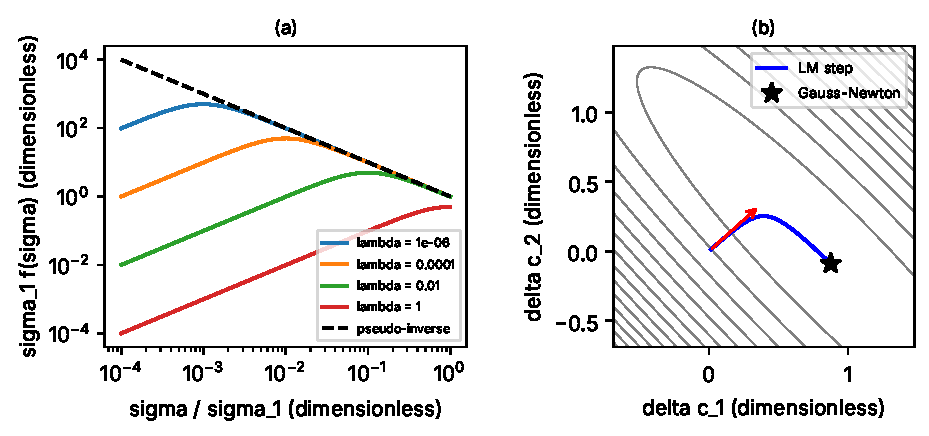
\includegraphics[width=0.98\linewidth]{figs/fitting_lmpath.pdf}
\caption{(a) Filter factors $\sigma_1 f(\sigma)=\sigma_1\sigma/(\sigma^2+\lambda\sigma_1^2)$ of the damped SVD step against $\sigma/\sigma_1$ (both dimensionless) for $\lambda=10^{-6},10^{-4},10^{-2},1$; the undamped pseudo-inverse $\sigma_1/\sigma$ is dashed. Damping caps the amplification of small singular directions. (b) Contours of a quadratic model $\tfrac12\norm{r-A\delta c}^2$ in the plane of a two-component step $(\delta c_1,\delta c_2)$, with an elongated valley. The arrow is the steepest-descent direction $A^\top r$ at the origin; the solid curve is the Levenberg--Marquardt step as the damping $\lambda'$ decreases from $10^{2}$ to $10^{-4}$, ending at the Gauss--Newton step (star).}
\label{fig:fitting-lmpath}
\end{figure}

\begin{checkpoint}
What happens to the LM step as $\lambda'\to\infty$: its length, and its direction?
\end{checkpoint}
\checkanswer{Its length tends to zero like $\norm{\hat A^\top\hat r}/\lambda'$, and its direction tends to the steepest-descent direction $\hat A^\top\hat r=-\nabla\Phi$.}

\begin{keyideas}
\item The gradient of $\Phi$ is $-\hat A^\top\hat r$; steepest descent is safe but slow.
\item The Levenberg--Marquardt step solves $(\hat A^\top\hat A+\lambda'I)\delta c=\hat A^\top\hat r$: Gauss--Newton for $\lambda'\to0$, short steepest descent for $\lambda'\to\infty$.
\item The LM matrix is positive definite for every $\lambda'>0$, so the step always exists and always points downhill; enough damping always produces a decrease unless the gradient vanishes.
\end{keyideas}

%==========================================================
\section{The damped step through the SVD}\label{sec:fitting-svd}

\subsection{Derivation}

Recall the singular value decomposition from Chapter~\ref{ch:least-squares}. Any real $n_{\rm fit}\times M$ matrix $\hat A$ of rank $p$ can be written
\begin{equation}
\hat A=\bm U\Sigma\bm V^\top,
\label{eq:fitting-svdA}
\end{equation}
where $\bm U$ is $n_{\rm fit}\times p$ with orthonormal columns $u_1,\dots,u_p$ ($\bm U^\top\bm U=I_p$), $\bm V$ is $M\times p$ with orthonormal columns $v_1,\dots,v_p$ ($\bm V^\top\bm V=I_p$), and $\Sigma=\mathrm{diag}(\sigma_1,\dots,\sigma_p)$ holds the positive singular values in decreasing order, $\sigma_1\ge\sigma_2\ge\cdots\ge\sigma_p>0$.

\begin{pitfall}
The paper's Appendix~A writes this decomposition with a plain $V$ for the matrix of right singular vectors. That $V$ has nothing to do with the potential $V(x)$. In this chapter we write the matrix in bold, $\bm V$, to keep them apart. (The paper overloads other letters too: $A$ is both this sensitivity matrix and, in Sec.~II~E, a non-Hermitian operator; $T$ is a training window, a tensor $T^{(n)}$, and a Chebyshev polynomial $T_k$.)
\end{pitfall}

\textbf{Claim.} The LM step is
\begin{equation}
\delta c=\bm V\,\mathrm{diag}\!\left(\frac{\sigma_i}{\sigma_i^2+\lambda'}\right)\bm U^\top\hat r .
\label{eq:fitting-svdstep}
\end{equation}

\textbf{Proof.} Call $D=\mathrm{diag}(\sigma_i/(\sigma_i^2+\lambda'))$ and $z=\bm VD\bm U^\top\hat r$. First compute the two sides of Eq.~\eqref{eq:fitting-lm} in SVD form:
\begin{align*}
\hat A^\top\hat A&=\bm V\Sigma\bm U^\top\bm U\Sigma\bm V^\top=\bm V\Sigma^2\bm V^\top\quad(\bm U^\top\bm U=I_p),\\
\hat A^\top\hat r&=\bm V\Sigma\bm U^\top\hat r .
\end{align*}
Now apply the LM matrix to $z$:
\begin{align*}
(\hat A^\top\hat A+\lambda'I)z&=\bm V\Sigma^2\bm V^\top\bm VD\bm U^\top\hat r+\lambda'\bm VD\bm U^\top\hat r\\
&=\bm V\Sigma^2D\bm U^\top\hat r+\bm V\lambda'D\bm U^\top\hat r\quad(\bm V^\top\bm V=I_p)\\
&=\bm V(\Sigma^2+\lambda'I_p)D\,\bm U^\top\hat r .
\end{align*}
The diagonal matrix $(\Sigma^2+\lambda'I_p)D$ has entries $(\sigma_i^2+\lambda')\cdot\sigma_i/(\sigma_i^2+\lambda')=\sigma_i$, so it equals $\Sigma$, and the right side is $\bm V\Sigma\bm U^\top\hat r=\hat A^\top\hat r$. Hence $z$ solves Eq.~\eqref{eq:fitting-lm}; since the LM matrix is invertible (Section~\ref{sec:fitting-lm}), the solution is unique and $\delta c=z$. $\blacksquare$

Read Eq.~\eqref{eq:fitting-svdstep} right to left, like a recipe: $\bm U^\top\hat r$ resolves the residual into its components $u_i^\top\hat r$ along the ``level patterns'' $u_i$; each component is multiplied by a \emph{filter factor} $f_i=\sigma_i/(\sigma_i^2+\lambda')$; and $\bm V$ converts the result into a change of coefficients along the ``coefficient patterns'' $v_i$. Without damping, $f_i=1/\sigma_i$, the pseudo-inverse of Chapter~\ref{ch:least-squares}.

\subsection{The paper's scaling: $\lambda'=\lambda\sigma_1^2$}

The paper measures damping relative to the largest singular value. It sets $\lambda'=\lambda\sigma_1^2$ with a dimensionless $\lambda$, so its step (Appendix~A step~6) is
\begin{equation}
c\;\mathrel{+}=\;\bm V\,\mathrm{diag}\!\left(\frac{\sigma_i}{\sigma_i^2+\lambda\sigma_1^2}\right)\bm U^\top r .
\label{eq:fitting-paperstep}
\end{equation}
(The symbol $\mathrel{+}=$ is programmers' shorthand for ``add the right side to $c$''.) Here we copy the paper's symbols; in our weighted convention read $r\to\hat r$ and take $\sigma_i$, $\bm U$ and $\bm V$ from the SVD of $\hat A$. Why the relative scaling? If every basis function is multiplied by a constant $\alpha$, then $\hat A\to\alpha\hat A$, every $\sigma_i\to\alpha\sigma_i$, and with $\lambda'=\lambda\sigma_1^2$ each filter factor becomes $\alpha\sigma_i/(\alpha^2\sigma_i^2+\lambda\alpha^2\sigma_1^2)=f_i/\alpha$. The step in coefficients shrinks by exactly $1/\alpha$, so the change $\delta V=\sum_k\delta c_k(\alpha\phi_k)$ is unchanged. A given value of $\lambda$ therefore means the same amount of damping whatever the units or normalization of the basis.

\subsection{What the filter does}

Four properties follow from $f(\sigma)=\sigma/(\sigma^2+\lambda\sigma_1^2)$.

\emph{Large singular values pass almost untouched.} For $\sigma^2\gg\lambda\sigma_1^2$, $f\approx1/\sigma$.

\emph{Small singular values are suppressed.} For $\sigma^2\ll\lambda\sigma_1^2$, $f\approx\sigma/(\lambda\sigma_1^2)\to0$, instead of the huge $1/\sigma$.

\emph{Amplification is capped.} $\dd f/\dd\sigma=[(\sigma^2+\lambda\sigma_1^2)-2\sigma^2]/(\sigma^2+\lambda\sigma_1^2)^2=(\lambda\sigma_1^2-\sigma^2)/(\sigma^2+\lambda\sigma_1^2)^2$, which vanishes at $\sigma=\sqrt\lambda\,\sigma_1$. There $f$ takes its largest value $\sqrt\lambda\sigma_1/(2\lambda\sigma_1^2)=1/(2\sqrt\lambda\,\sigma_1)$. No component of the residual is ever amplified by more than this.

\emph{The step shrinks as damping grows.} Since the $v_i$ are orthonormal, $\norm{\delta c}^2=\sum_if_i^2(u_i^\top\hat r)^2$, and every $f_i$ decreases as $\lambda$ increases (its denominator grows). So $\norm{\delta c}$ decreases steadily with $\lambda$.

\begin{sample}{Filter factors}
A sensitivity matrix has singular values $\sigma=(10,\ 1,\ 0.01)$ and the damping is $\lambda=0.01$. Compute the filter factors and compare with the pseudo-inverse.

\emph{Step 1: the damping term.} $\lambda\sigma_1^2=0.01\times100=1$.

\emph{Step 2: the factors.} $f_1=10/(100+1)=0.0990$, $f_2=1/(1+1)=0.5$, $f_3=0.01/(0.0001+1)=0.0099990$.

\emph{Step 3: compare.} The pseudo-inverse would use $1/\sigma=(0.1,\ 1,\ 100)$.

\emph{Step 4: the cap.} The largest possible factor is $1/(2\sqrt\lambda\sigma_1)=1/(2\times0.1\times10)=0.5$, reached at $\sigma=\sqrt\lambda\sigma_1=1$.
\[
\boxed{f=(0.0990,\ 0.5,\ 0.0100)\ \text{instead of}\ (0.1,\ 1,\ 100)}
\]
The weakest direction, which the pseudo-inverse would amplify 100-fold, is now multiplied by one hundredth.
\end{sample}

\subsection{Too many coefficients}

When $M>n_{\rm fit}$ the rank $p$ is at most $n_{\rm fit}$, and $\bm V$ has only $p$ columns. Every step Eq.~\eqref{eq:fitting-svdstep} is a combination of $v_1,\dots,v_p$, the directions in coefficient space that actually move some level. The remaining $M-p$ directions (the \emph{null space} of $\hat A$, Chapter~\ref{ch:least-squares}) change no level to first order, and the step never moves along them. As $\lambda\to0$ the step becomes the minimum-norm step of Chapter~\ref{ch:least-squares}, as in the Sample Problem ``One linearized step in the box''. Because $\hat A$ changes from iterate to iterate, the final $c$ after many steps is not exactly the minimum-norm solution of anything; it depends on the path.

\subsection{The ridge variant}

The paper also runs fits with a ``ridge variant'' that ``adds $\mu\Sigma_1^2$ to the filter denominator'' (Appendix~A step~6), with ridge strength $\mu=0.03$ or $0.3$ (Table~I). Taken literally, the step becomes
\begin{equation}
c\;\mathrel{+}=\;\bm V\,\mathrm{diag}\!\left(\frac{\sigma_i}{\sigma_i^2+(\lambda+\mu)\sigma_1^2}\right)\bm U^\top r ,
\label{eq:fitting-ridgestep}
\end{equation}
which is an LM step whose damping can never fall below $\mu$. Compare the Tikhonov (ridge) regularization of Chapter~\ref{ch:least-squares}, which adds a penalty $\tfrac12\mu\sigma_1^2\norm{c}^2$ on the coefficients themselves and so changes \emph{where} the minimum is. The two are not the same. Under this literal reading of the record, the step of Eq.~\eqref{eq:fitting-ridgestep} vanishes exactly where the unregularized gradient vanishes, so the stationary points are unchanged; the variant acts by shortening steps, which, combined with the accept rule and iteration cap of Section~\ref{sec:fitting-schedule}, stops the iteration closer to its starting point $c=0$. This is our reading of the one-line description in the record; Problem~23 works out the difference, and the scripts in \cite{zenodo} are the authority on the exact implementation.

\begin{keyideas}
\item The LM step in SVD form: $\delta c=\bm V\,\mathrm{diag}(\sigma_i/(\sigma_i^2+\lambda'))\bm U^\top\hat r$, proved by substitution.
\item The paper uses $\lambda'=\lambda\sigma_1^2$, which makes $\lambda$ independent of how the basis is normalized.
\item Filter factors pass strong directions, suppress weak ones, and never exceed $1/(2\sqrt\lambda\sigma_1)$; the step length falls as $\lambda$ rises.
\item With $M>n_{\rm fit}$ the step only moves within the span of $v_1,\dots,v_p$.
\item Read literally, the paper's ridge variant raises the floor of the damping, which would differ from a Tikhonov penalty on $c$; the archived scripts decide.
\end{keyideas}

%==========================================================
\section{The paper's damping schedule, line by line}\label{sec:fitting-schedule}

An LM method needs a rule for choosing $\lambda$ at each iteration. Here is the paper's rule, quoted from Appendix~A step~6 (with the revision settings stated just after step~15, ``start $c=0$, at most 60 iterations, acceptance $0.999$''):

\begin{quote}
iterate \{eigensolve with vectors; $A_{nk}=\int|\psi_n|^2\phi_k$; SVD-damped step $c\mathrel{+}=V(\Sigma/(\Sigma^2+\lambda\Sigma_1^2))U^\top r$ with try-list $(0.2\lambda,\lambda,5\lambda,25\lambda)$; on success $\lambda\leftarrow\max(0.5\lambda_{\rm acc},10^{-7})$, on total failure $\lambda\leftarrow30\lambda$, stop at $\lambda>10^4$; accept only improvements ($\times0.999$; the scale-2 $M{=}300$ row used $1-10^{-5}$)\}
\end{quote}

\Cref{tab:fitting-schedule} translates each clause.

\begin{table}[htbp]\centering
\caption{The clauses of the paper's fitting loop (Appendix~A step~6) and what each one does.}
\label{tab:fitting-schedule}
\small
\begin{tabular}{p{0.36\linewidth}p{0.56\linewidth}}
\toprule
clause & meaning\\
\midrule
eigensolve with vectors & compute $E_n$ and eigenvectors $w_n$ of $H(c)$ for the fitted levels (Chapter~\ref{ch:finite-differences})\\
$A_{nk}=\int|\psi_n|^2\phi_k$ & build the sensitivity matrix, Eq.~\eqref{eq:fitting-Adisc}\\
SVD-damped step & Eq.~\eqref{eq:fitting-paperstep}: one SVD per iteration, then each trial step costs only a few matrix products plus one eigenvalue-only solve to score it\\
try-list $(0.2\lambda,\lambda,5\lambda,25\lambda)$ & candidate damping values, from bolder to more cautious\\
accept only improvements ($\times0.999$) & a trial is accepted only if its rms is below $0.999$ times the current rms\\
on success $\lambda\leftarrow\max(0.5\lambda_{\rm acc},10^{-7})$ & $\lambda_{\rm acc}$ is the damping of the accepted trial; next time start bolder, but never below $10^{-7}$\\
on total failure $\lambda\leftarrow30\lambda$ & no trial accepted: keep $c$, damp much harder\\
stop at $\lambda>10^4$ & give up when even very short steps cannot improve by $0.1\%$\\
at most 60 iterations & a cap on the number of passes through the loop (stated for the revision computations, App.~A after step~15; not stated for the original fits)\\
\bottomrule
\end{tabular}
\end{table}

Two details are not spelled out in the quoted text: the initial value of $\lambda$, and whether the try-list is scanned in order with the first acceptable trial taken, or all four are evaluated and the best taken. In this book's reading, and in our code, the list is scanned in order and the first trial that passes is accepted, and we start from $\lambda=1$; both are our choices, and the archived scripts \cite{zenodo} record the paper's. The logic of the schedule is the same either way.

\subsection{Why the schedule works}

The accept rule makes the in-sample rms a non-increasing sequence: $c$ changes only when the rms drops by at least $0.1\%$. The try-list explores a factor of $125$ in damping around the current $\lambda$ at the cost of at most four eigenvalue solves (each trial needs only eigenvalues, not eigenvectors). After a success the next iteration starts at half the accepted damping, so the algorithm grows bolder while things go well and approaches Gauss--Newton speed. After a total failure, $\lambda$ jumps by 30, and by Section~\ref{sec:fitting-lm} enough damping always produces a decrease unless the gradient vanishes.

The threshold $0.999$ also provides the stopping mechanism. Near a minimum, any improvement available is tiny; the trials fail the $0.1\%$ test, $\lambda$ is multiplied by 30 again and again, and once it exceeds $10^4$ the loop stops. A stricter threshold stops earlier, a looser one later. The paper reports one case where this matters: the scale-2 $M=300$ row of Table~I ``required relaxing the step-acceptance threshold; under the strict protocol the optimizer accepts no step at all'' (Table~I caption), and it used $1-10^{-5}$ instead.

\begin{pycode}
import numpy as np

def lm_fit(c, resid, jac, lam=1.0, maxiter=60, accept=0.999):
    # resid(c): r_n/gap_n;  jac(c): A_nk/gap_n  (paper App. A, step 6)
    r = resid(c)
    cur = np.sqrt(np.mean(r**2))                 # current rms
    for it in range(maxiter):
        U, s, Vt = np.linalg.svd(jac(c), full_matrices=False)
        Utr = U.T @ r
        accepted = False
        for lam_try in (0.2*lam, lam, 5*lam, 25*lam):
            f = s / (s**2 + lam_try * s[0]**2)    # filter factors
            c_try = c + Vt.T @ (f * Utr)          # Vt.T is the matrix V
            r_try = resid(c_try); rms_try = np.sqrt(np.mean(r_try**2))
            if rms_try < accept * cur:            # accept only improvements
                c, r, cur = c_try, r_try, rms_try
                lam = max(0.5 * lam_try, 1e-7)
                accepted = True
                break
        if not accepted:                           # total failure
            lam = 30 * lam
            if lam > 1e4:
                break                              # stop rule
    return c, cur

# example: two-level model, target 0.5, start c = 0.5
Em = lambda c: 2 - np.sqrt(1 + c[0]**2)
res = lambda c: np.array([0.5 - Em(c)])
jac = lambda c: np.array([[-c[0] / np.sqrt(1 + c[0]**2)]])
print(lm_fit(np.array([0.5]), res, jac))  # c close to 1.118034, rms near 0
\end{pycode}

The example call fits the two-level model of Section~\ref{sec:fitting-gn}. It returns a coefficient within $10^{-6}$ of the exact answer $c_*=1.118034$ and an rms that is zero to within rounding; with \texttt{maxiter=1} it returns $c=1.21175$, the single iteration worked out by hand in the Sample Problem ``One pass of the schedule on the two-level model''.

\begin{sample}{One pass of the schedule on the two-level model}
Run the first iteration of the schedule (code above) on the two-level model of Section~\ref{sec:fitting-gn}, starting from $c=0.5$ with $\lambda=1$. There is one parameter, so the ``SVD'' of the $1\times1$ matrix $J$ has $\sigma_1=|J|$.

\emph{Step 1: current state.} From the Sample Problem ``Gauss--Newton on the two-level model'', $r=-0.381966$, $J=-0.447214$, $\sigma_1^2=J^2=0.2$. The current rms is $|r|=0.381966$, and a trial passes only if its rms is below $0.999\times0.381966=0.381584$.

\emph{Step 2: first trial.} $\lambda_{\rm try}=0.2\lambda=0.2$, so the effective damping is $\lambda'=\lambda_{\rm try}\sigma_1^2=0.04$. By the Sample Problem ``Damped steps on the two-level model'' this gives $\delta c=0.71175$, $c=1.21175$, and $|r|=0.071095$.

\emph{Step 3: the test.} $0.071095<0.381584$, so the trial is accepted and the remaining trials are not tried.

\emph{Step 4: update the damping.} $\lambda\leftarrow\max(0.5\times0.2,\,10^{-7})=0.1$.
\[
\boxed{c=1.21175,\quad \mathrm{rms}=0.0711,\quad \lambda=0.1\ \text{after one iteration}}
\]
The next iteration starts with trial damping $0.02$, close to Gauss--Newton, which is appropriate because the iterate is now near the solution.
\end{sample}

\subsection{Random restarts}

The paper's protocol ``is deterministic from $c=0$; optimizer variability is probed with randomized initial $c$'' (Sec.~II~C). Starting from a random $c^{(0)}$ instead of $0$ tests whether the answer depends on where the descent began. The two-level model shows why it might: \Cref{fig:fitting-landscape} has two minima, and the one you reach depends on the sign of the starting $c$. In a problem with hundreds of coefficients the landscape can have many valleys, and an LM method only ever finds a point where the gradient is (nearly) zero near where it started. The paper reports that four random-init repeats of the scale-1, $M=400$, zeros 1--400 configuration ``give identical in-sample rms $0.1370$ and OOS $0.365$--$0.379$'' (Table~I caption): the in-sample error did not depend on the start, but the held-out behavior varied a little. That pattern (many different coefficient vectors that fit equally well) is what you expect when there are far more ways to fit the data than data, a theme of Chapter~\ref{ch:generalization}.

\begin{checkpoint}
Why does the accept rule guarantee that the final in-sample rms is never worse than the starting one?
\end{checkpoint}
\checkanswer{$c$ is changed only when a trial's rms is below $0.999$ times the current rms. So the sequence of accepted rms values strictly decreases, and if nothing is ever accepted the final $c$ is the starting $c$.}

\begin{keyideas}
\item Each iteration: one eigensolve with vectors, one SVD, then up to four trial steps needing only eigenvalues.
\item Accept a trial only if it lowers the rms by at least $0.1\%$; after success relax damping to half the accepted value, after total failure multiply it by 30; stop when $\lambda>10^4$ (and, in the revision computations, after at most 60 iterations).
\item Random starting points probe whether the result depends on the optimizer's path.
\end{keyideas}

%==========================================================
\section{Three bases for $\delta V$}\label{sec:fitting-bases}
% DYK-BEGIN
\begin{didyouknow}{Runge's Wiggles}
In 1901 Carl Runge showed that fitting a polynomial through more and more \emph{equally spaced} points can make things worse. For $1/(1+25x^2)$ on $[-1,1]$, the interpolating polynomials oscillate wildly near the ends, and the error grows without bound. Clustering the points toward the ends, as Chebyshev nodes do, cures the problem. The choice of basis and sampling can make or break a fit.
\end{didyouknow}
% DYK-END

The choice of basis functions $\phi_k$ decides which shapes $\delta V$ can take. The Wu--Sprung background is even, $V(-x)=V(x)$, and the paper keeps the correction even too, so that the fitted potential stays even and its states keep definite parity (Chapter~\ref{ch:bound-states}). All three bases below are even functions of $x$. \Cref{fig:fitting-bases} plots the first few members of each.

\paragraph{Cosines.} $\phi_k(x)=\cos(k\pi x/L)$, $k=0,1,\dots,M-1$. By Chapter~\ref{ch:fourier-series} these are orthogonal on $[-L,L]$ and form the natural Fourier basis for even functions. Each is spread over the whole box (a \emph{global} basis), with uniform resolution: member $k$ has wavelength $2L/k$ everywhere.

\paragraph{Chebyshev polynomials.} The Chebyshev polynomials $T_k(y)$ on $-1\le y\le1$ are defined by
\begin{equation}
T_k(y)=\cos(k\arccos y),
\label{eq:fitting-cheb}
\end{equation}
that is, if $y=\cos\theta$ with $0\le\theta\le\pi$, then $T_k(y)=\cos k\theta$. They are polynomials: $T_0=1$, $T_1=y$, and from the identity $\cos((k+1)\theta)+\cos((k-1)\theta)=2\cos\theta\cos k\theta$ we get the recurrence $T_{k+1}(y)=2yT_k(y)-T_{k-1}(y)$, giving $T_2=2y^2-1$, $T_3=4y^3-3y$. The paper uses $\phi_k(x)=T_k(2|x|/L-1)$, $k=0,\dots,M-1$: the variable $y=2|x|/L-1$ runs from $-1$ at $x=0$ to $+1$ at $|x|=L$. Since $y=\cos\theta$ changes slowly near $\theta=0$ and $\theta=\pi$, equal steps in $\theta$ crowd together near $y=\pm1$; the oscillations of $T_k$ are therefore densest near $x=0$ and $|x|=L$. This is the paper's ``resolution concentrated near $x=0$ and $x=L$'' (Sec.~II~C, ``Other bases''). The absolute value makes $\phi_k$ even, at the price of a kink at $x=0$ for every $k\ge1$. To see this, differentiate $T_k(\cos\theta)=\cos k\theta$ with respect to $\theta$: $T_k'(y)\,(-\sin\theta)=-k\sin k\theta$, so $T_k'(y)=k\sin k\theta/\sin\theta$. As $y\to-1$, $\theta\to\pi$ and both sines vanish; l'H\^opital's rule gives $T_k'(-1)=k\cdot k\cos k\pi/\cos\pi=(-1)^{k+1}k^2$. Just right of $x=0$, $\dd\phi_k/\dd x=(2/L)T_k'(y)\to(2/L)(-1)^{k+1}k^2$; by evenness the slope just left of $x=0$ is the negative of this, so the slope jumps by $4k^2/L\neq0$ (visible in \Cref{fig:fitting-bases}).

\paragraph{Hat functions.} Put $M$ equally spaced nodes $u_j=j/(M-1)$, $j=0,\dots,M-1$, on the interval $0\le u\le1$, where $u=|x|/L$. (The paper says only ``$M$ uniform nodes of $|x|/L$'' and does not specify their placement; we take nodes that include both ends, and the archived scripts \cite{zenodo} record the paper's choice. The variable $u$ and the nodes $u_j$ have nothing to do with the left singular vectors $u_i$ of Section~\ref{sec:fitting-svd}.) The hat function centered at node $j$ is
\begin{equation}
\phi_j(x)=\max\Bigl(0,\;1-(M-1)\bigl|u-u_j\bigr|\Bigr),\qquad u=\frac{|x|}{L}.
\label{eq:fitting-hat}
\end{equation}
It equals 1 at its own node, 0 at every other node, and is a straight line in between neighbors. A combination $\sum_jc_j\phi_j$ is the piecewise-linear function that passes through the values $c_j$ at the nodes. Hats are \emph{local}: each is nonzero only within one node spacing of its center, so a coefficient changes the potential only in one small region. The paper calls this ``the simplest stand-in for a wavelet-type basis''. Hats sum to one: if $u$ lies between nodes $u_j$ and $u_{j+1}$, only $\phi_j$ and $\phi_{j+1}$ are nonzero there, equal to $1-(M-1)(u-u_j)$ and $1-(M-1)(u_{j+1}-u)$; their sum is $2-(M-1)(u_{j+1}-u_j)=2-1=1$.

\begin{figure}[htbp]\centering
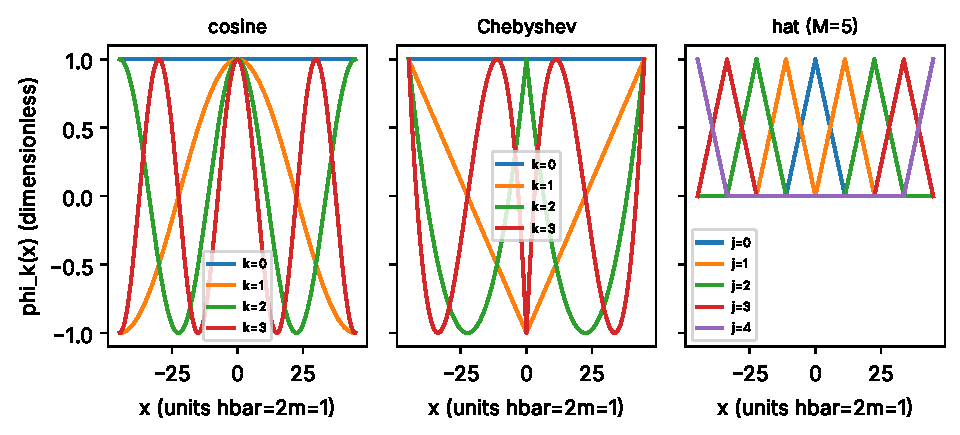
\includegraphics[width=0.98\linewidth]{figs/fitting_bases.pdf}
\caption{The three even bases used for $\delta V$ in the paper, on $[-L,L]$ with $L=44.883$ (units $\hbar=2m=1$; $\phi$ is dimensionless). Left: cosines $\cos(k\pi x/L)$, $k=0,\dots,3$. Middle: Chebyshev polynomials $T_k(2|x|/L-1)$, $k=0,\dots,3$, with kinks at $x=0$ for every $k\ge1$. Right: the five hat functions for $M=5$ nodes in $|x|/L$.}
\label{fig:fitting-bases}
\end{figure}

\begin{sample}{Evaluating Chebyshev and hat functions}
(a) Evaluate $\phi_3(x)=T_3(2|x|/L-1)$ at $x=L/4$ two ways. (b) For $M=5$ hats, find all nonzero $\phi_j$ at $|x|/L=0.6$.

\emph{Step 1: the variable.} At $x=L/4$, $y=2\cdot\tfrac14-1=-\tfrac12$.

\emph{Step 2: polynomial.} $T_3(-\tfrac12)=4(-\tfrac18)-3(-\tfrac12)=-\tfrac12+\tfrac32=1$.

\emph{Step 3: cosine form.} $\arccos(-\tfrac12)=2\pi/3$, so $T_3=\cos(3\cdot2\pi/3)=\cos2\pi=1$. The two agree.

\emph{Step 4: hats.} Nodes are $0,0.25,0.5,0.75,1$, and $M-1=4$. Only the neighbors $u_2=0.5$ and $u_3=0.75$ are within $0.25$ of $0.6$: $\phi_2=1-4(0.1)=0.6$, $\phi_3=1-4(0.15)=0.4$.
\[
\boxed{T_3(-\tfrac12)=1;\qquad \phi_2=0.6,\ \phi_3=0.4,\ \text{others }0\ (\text{sum }1)}
\]
\end{sample}

\begin{keyideas}
\item Cosines: global, orthogonal, uniform resolution.
\item Chebyshev $T_k(2|x|/L-1)$: global, resolution concentrated near $x=0$ and $|x|=L$.
\item Hats: local piecewise-linear functions on $M$ nodes of $|x|/L$; they sum to one.
\item All three are even, so the fitted potential stays even; only the basis changes between the paper's three families.
\end{keyideas}

%==========================================================
\section{The coverage law: how many basis functions are enough?}\label{sec:fitting-coverage}

\subsection{Which cosines can push which levels}

The Wu--Sprung panel of \Cref{fig:fitting-sensitivity} shows that level $n$ responds to cosines up to a cutoff. We now derive that cutoff heuristically. The argument uses the WKB picture of Chapter~\ref{ch:wkb} and is approximate, not a theorem.

\emph{Step 1: the WKB density.} A warning on notation first: in this section $k(x)$ is the local wavenumber, a function of position, while the basis index of $\cos(k\pi x/L)$ is a plain integer $k$; to keep them apart we write the cosine's wavenumber as $q=k\pi/L$. Recall from Chapter~\ref{ch:wkb} that between its turning points (the points where $E=V(x)$, at which a classical particle would stop and turn back) a level of energy $E$ has local wavenumber $k(x)=\sqrt{E-V(x)}$ and WKB wavefunction $\psi\approx C\,k(x)^{-1/2}\cos\bigl(\theta(x)\bigr)$, where $\theta(x)=\int^xk(x')\,\dd x'-\pi/4$ and $C$ is a constant. (The wave has the local wavelength $2\pi/k(x)$ set by the classical momentum; the amplitude factor $k^{-1/2}$ makes $|\psi|^2$ proportional to the time a classical particle spends near $x$; the phase $-\pi/4$ comes from the connection formulas of Chapter~\ref{ch:wkb}.) Squaring and using $\cos^2\theta=\tfrac12(1+\cos2\theta)$,
\[
|\psi|^2\approx\frac{C^2}{2k(x)}\Bigl[1+\cos2\theta(x)\Bigr].
\]
The density is a slowly varying part plus a ripple whose phase $2\theta$ advances at the local rate $\dd(2\theta)/\dd x=2k(x)$. So the ripple has local wavenumber $2k(x)$.

\emph{Step 2: overlap with one cosine.} The sensitivity $A_{nk}=\int|\psi_n|^2\cos(qx)\,\dd x$ with $q=k\pi/L$ has two pieces. The slow part of $|\psi|^2$ overlaps only with cosines of low $q$. The ripple contributes $\int\frac{C^2}{2k}\cos2\theta\cos qx\,\dd x=\frac{C^2}{4}\int\frac1k\bigl[\cos(2\theta-qx)+\cos(2\theta+qx)\bigr]\dd x$. Each integrand oscillates rapidly, and its positive and negative lobes cancel, except near a point where its phase is stationary, $\dd(2\theta-qx)/\dd x=2k(x)-q=0$. This is called \emph{stationary-phase} reasoning. A small example shows why the stationary point dominates. With a phase that never stands still, $\int_{-X}^{X}\cos(ax)\,\dd x=\bigl[\sin(ax)/a\bigr]_{-X}^{X}=2\sin(aX)/a$, at most $2/a$ in size: the lobes cancel and only an endpoint remnant of order $1/a$ survives. With the phase $ax^2$, which is stationary at $x=0$, the integrand $\cos(ax^2)$ stays positive throughout $ax^2<\pi/2$, a central interval of width $2\sqrt{\pi/2a}$ that shrinks only like $1/\sqrt a$; this uncancelled region contributes an amount of order $1/\sqrt a$, far more than $1/a$ when $a$ is large. For $a=100$ and $X=3$ the first integral is at most $0.02$ in size, while numerically the second is about $0.13$.

\begin{beyond}
The infinite-range value $\int_{-\infty}^{\infty}\cos(ax^2)\,\dd x=\sqrt{\pi/2a}$ (about $0.125$ for $a=100$) is a Fresnel integral, and the general statement that an oscillatory integral is dominated by its points of stationary phase is the method of stationary phase. We take both on trust; they are treated with the method of steepest descents in \cite{rhb}.
\end{beyond}

\emph{Step 3: the cutoff.} A matching point $2k(x)=q$ exists only if $q$ is no larger than the maximum of $2k(x)$. For a well with its minimum $V_0$ at $x=0$, that maximum is $2\sqrt{E-V_0}$. Hence level $n$ responds strongly only to cosines with
\begin{equation}
\frac{k\pi}{L}\;\lesssim\;2\sqrt{E_n-V_0},
\label{eq:fitting-reach}
\end{equation}
which is the dashed curve of \Cref{fig:fitting-sensitivity}. Above the cutoff the condition $2k(x)=q$ has no real solution anywhere in the well, so the positive and negative lobes of the integrand cancel along the whole range of integration and the overlap is small, though not exactly zero. That is why the figure shows a sharp fall, not a hard edge.

\begin{beyond}
How small is the overlap above the cutoff? A refinement of the stationary-phase method, the method of steepest descents, treats the condition $2k(x)=q$ as an equation for a \emph{complex} $x$ and shows that above the cutoff the overlap decreases exponentially as $q$ grows. We take this on trust; the method is developed in the chapter on asymptotic expansions of \cite{rhb}. In this chapter we use only the qualitative statement that the overlap is small above the cutoff, which is what \Cref{fig:fitting-sensitivity} shows.
\end{beyond}

\emph{Check against the box.} With $V_0=0$ and $E_n=(n\pi/2L)^2$, Eq.~\eqref{eq:fitting-reach} reads $k\pi/L\lesssim n\pi/L$, i.e.\ $k\lesssim n$. The Sample Problem ``The sensitivity matrix of the box'' found the exact answer: in the box only $k=n$ (and $k=0$) respond. The box is special because its ripple has a single wavenumber everywhere, so only the matching cosine survives; in the Wu--Sprung well $2k(x)$ ranges from 0 at the turning points up to $2\sqrt{E-V_0}$, and every cosine in that range finds a matching point.

\subsection{The law}

To move each of the levels up to $E_{\max}$ independently of its neighbors, the basis must contain cosines that reach the finest ripple of the top level. The largest wavenumber in a basis of $M$ cosines is $(M-1)\pi/L\approx M\pi/L$. So the basis is effectively complete for joint level shifts up to $E_{\max}$ when
\begin{equation}
\frac{M\pi}{L}\;>\;2\sqrt{E_{\max}} ,
\label{eq:fitting-coverage}
\end{equation}
which is the paper's coverage law (Sec.~III, first paragraph). We have used $\sqrt{E}$ rather than $\sqrt{E-V_0}$, as the paper does; for small $u$ the first-order Taylor expansion $\sqrt{1-u}\approx1-u/2$ gives $\sqrt{E-V_0}=\sqrt E\,\sqrt{1-V_0/E}\approx\sqrt E\,(1-V_0/2E)$, so the relative difference is about $V_0/(2E)$. At the top scored level, $E\approx811$, that is $0.6\%$, so the paper's form is harmless where the law matters. At the bottom of the spectrum the difference is large (at $E=t_1=14.13$, $\sqrt{E-V_0}\approx0.56\sqrt E$), but the coverage law is set by the highest level, not the lowest. Two further conditions are implicit: you also need at least as many coefficients as levels, $M\ge n_{\rm fit}$, to shift $n_{\rm fit}$ levels independently, and the optimizer must actually find the fit. Equation~\eqref{eq:fitting-coverage} is a heuristic rule of thumb, derived from WKB and stationary phase, not a proven statement about the minimum of $\Phi$. In particular it is not a necessary condition for a small in-sample error. It concerns shifting \emph{all consecutive} levels up to $E_{\max}$ independently. A level above the reach of the basis still responds to all $M$ cosines (its own cutoff lies above $M$), so if only some levels are fitted (every other one, say), or if $n_{\rm fit}$ is well below $M$, the sensitivity matrix can still have full row rank and the fit can reach very small residuals even though $M\pi/L<2\sqrt{E_{\max}}$. The paper's Table~III shows this: at scale 1, $M=400$ fits the 200 odd-indexed (or even-indexed) zeros among zeros 1--400 to rms $<10^{-3}$, whereas covering all consecutive levels up to $t_{400}\approx679.7$ would, by Eq.~\eqref{eq:fitting-coverage}, need $M\gtrsim745$.

\begin{figure}[htbp]\centering
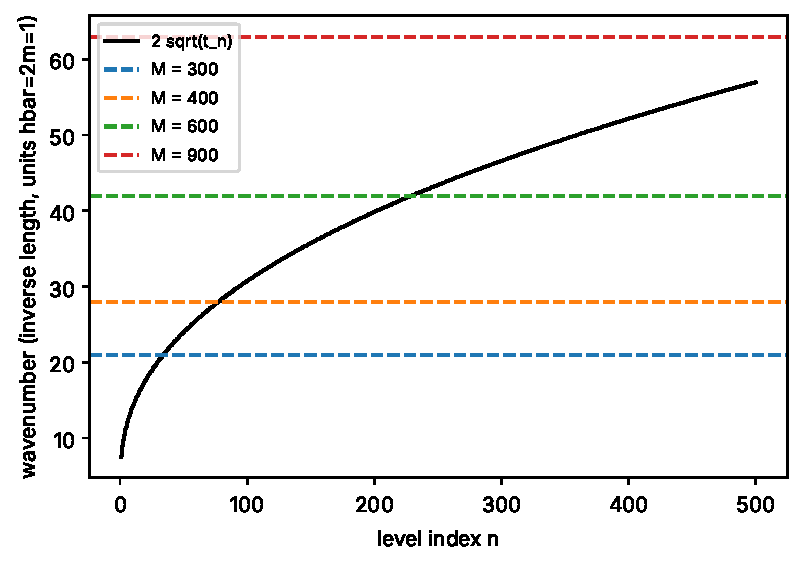
\includegraphics[width=0.85\linewidth]{figs/fitting_coverage.pdf}
\caption{Coverage law at scale 1 ($L=44.883$, units $\hbar=2m=1$). Solid curve: the finest ripple wavenumber $2\sqrt{t_n}$ of level $n$ (in units of inverse length), using the zero heights $t_n$ as the level energies. Horizontal lines: the highest cosine wavenumber $M\pi/L$ for $M=300,400,600,900$. A basis covers all levels below the crossing point; only $M=900$ clears all 500 scored levels.}
\label{fig:fitting-coverage}
\end{figure}

\begin{sample}{How many cosines for 500 zeros?}
At scale 1 ($L=44.883$) the top scored level is $t_{500}=811.1843588465$ (paper Appendix~A, ``Key anchors''). (a) How many cosines does Eq.~\eqref{eq:fitting-coverage} require? (b) Up to which energy, and roughly which level index, does $M=400$ reach?

\emph{Step 1: required wavenumber.} $2\sqrt{811.18}=2\times28.481=56.96$.

\emph{Step 2: required $M$.} $M>56.96\,L/\pi=56.96\times44.883/3.14159=813.8$.

\emph{Step 3: reach of $M=400$.} Solving $400\pi/L=2\sqrt{E}$ gives $E=(400\pi/2L)^2=(13.999)^2=196.0$.

\emph{Step 4: level index.} The number of zeros below $196$ is approximately $\Nsm(196)=\frac{196}{2\pi}\log\frac{196}{2\pi}-\frac{196}{2\pi}+\frac78\approx77.0$.
\[
\boxed{M\gtrsim 814\ \text{for all 500 levels};\quad M=400\ \text{gives full coverage only up to }E\approx196,\ \text{about level }77}
\]
``Full coverage'' means that every consecutive level up to that energy can be shifted independently. Levels above $E\approx196$ still respond to all 400 cosines, so the law does not say they cannot be fitted; it says only that $M=400$ does not guarantee independent shifts of every consecutive level there.
This is consistent with the paper: $M=900$ reproduces all 500 zeros to rms $<10^{-4}$, while $M=300$ leaves $0.186$ (Sec.~III).
\end{sample}

\begin{checkpoint}
An $M=400$ cosine fit on zeros 1--400 reaches in-sample rms $0.137$ (Table~I). By the coverage law, which levels would you expect to be fitted well and which poorly?
\end{checkpoint}
\checkanswer{The law alone does not tell you. It guarantees independent shifts only for the consecutive levels up to about level 77. Levels above that still respond to all 400 cosines, and with as many coefficients as training levels the sensitivity matrix can have full row rank, so they may well be fitted too. The law is heuristic and is not a necessary condition for a small error: Table~III shows $M=400$ fitting 200 odd-indexed levels as high as $n=399$ to rms $<10^{-3}$. Where the residual of the 1--400 fit is concentrated can only be found by computing it, which this chapter does not do.}

\subsection{In-sample error can only fall with $M$}

The paper reports that ``in-sample error falls steadily with basis size $M$'' (Fig.~3 caption) in every basis (Table~II). Here is the reason, and its limit. The bases are \emph{nested}: the cosine family with $M$ members is contained in the family with $M+1$ members (set $c_M=0$). Every potential available with $M$ coefficients is available with $M+1$, so the smallest achievable $\Phi$ cannot increase with $M$. For hats, the families with different $M$ are not exactly nested (node positions move), so the argument holds only approximately. And the argument is about the \emph{best} fit; an optimizer that stops early could, in principle, report a larger error at larger $M$. \Cref{fig:fitting-toyfit} shows the steady fall in a small toy problem you can run in seconds.

\begin{figure}[htbp]\centering
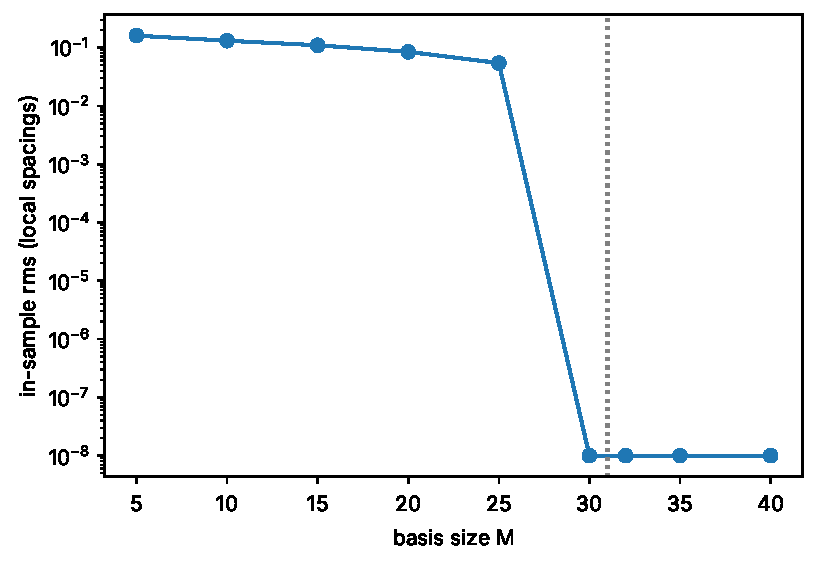
\includegraphics[width=0.85\linewidth]{figs/fitting_toyfit.pdf}
\caption{Toy version of the paper's fit: a box of half-width $L=10$ with $V=0$ on $N=300$ grid points (units $\hbar=2m=1$), cosine basis, and targets equal to the lowest 30 levels displaced by random amounts of rms $0.2$ local spacings (seed 0). The paper-style damped schedule of Section~\ref{sec:fitting-schedule} is run for each basis size $M$. In-sample rms (in local spacings, log scale) falls with $M$ and collapses to essentially zero once $M$ reaches the number of fitted levels, $M=30$, where the first-order equations first become exactly solvable (Problem~24).}
\label{fig:fitting-toyfit}
\end{figure}

\begin{keyideas}
\item By WKB and stationary phase, level $n$ responds to cosines with $k\pi/L\lesssim2\sqrt{E_n-V_0}$ (heuristic).
\item Coverage law: $M\pi/L>2\sqrt{E_{\max}}$ makes the cosine family effectively complete for joint shifts of all levels up to $E_{\max}$; at scale 1 this needs $M\gtrsim814$.
\item For nested bases the best achievable in-sample error cannot rise with $M$.
\item Coverage is about what can be fitted, not about what will be predicted.
\end{keyideas}

%==========================================================
\section{Paper connection}\label{sec:fitting-paper}

\paragraph{Sec.~II~C, first paragraph.} The paper writes $\delta V(x)=\sum_{k=0}^{M-1}c_k\cos(k\pi x/L)$ (our Eq.~\eqref{eq:fitting-deltaV}), forms residuals $r_n=\tilde t_n-E_n$ (Eq.~\eqref{eq:fitting-residual}) and ``the first-order sensitivity $A_{nk}=\int|\psi_n|^2\cos(k\pi x/L)\,dx$'' (Eq.~\eqref{eq:fitting-A}, Section~\ref{sec:fitting-sensitivity}), and updates ``$c$ by SVD-damped least squares with a Levenberg--Marquardt schedule, accepting only steps that improve the rms''. You can now read each phrase: the SVD step is Eq.~\eqref{eq:fitting-paperstep}, its derivation from damped least squares is Sections~\ref{sec:fitting-lm}--\ref{sec:fitting-svd}, and the schedule is \Cref{tab:fitting-schedule}. ``Iterated linearization'' is Gauss--Newton (Section~\ref{sec:fitting-gn}) made safe by damping.

\paragraph{Appendix~A step~6.} Every symbol of the step $c\mathrel{+}=V(\Sigma/(\Sigma^2+\lambda\Sigma_1^2))U^\top r$ has been defined: the plain $V$ there is our $\bm V$ of right singular vectors, $\Sigma_1$ is $\sigma_1$, and the ridge variant ``adds $\mu\Sigma_1^2$ to the filter denominator'' (literal reading: Eq.~\eqref{eq:fitting-ridgestep}). Appendix~A step~9 states the normalization $\sum\psi^2dx=1$ used in our Eq.~\eqref{eq:fitting-Adisc}. Step~7, ``plain eigensolve of the fitted potential, scored on held-out zeros'', is the out-of-sample evaluation; it uses no part of the fitting machinery except the final $c$.

\paragraph{Sec.~II~C, "Other bases"; Table~II.} The three bases of Section~\ref{sec:fitting-bases} are exactly the paper's: cosines, $T_k(2|x|/L-1)$, and hats ``on $M$ uniform nodes of $|x|/L$''. ``Only the basis changes.'' Table~II's in-sample column falls with $M$ in each basis (Chebyshev $0.230,0.162,0.111$; hat $0.221,0.145,0.066$ at $M=200,400,600$), as Section~\ref{sec:fitting-coverage} predicts for the best achievable error in the nested cosine and Chebyshev families, and approximately for hats.

\paragraph{Sec.~III, first paragraph.} ``On the full 500 zeros the fit reaches rms $0.186$ at $M=300$ and reproduces all 500 zeros to rms $<10^{-4}$ spacings by $M=900$, consistent with a basis-coverage law (the cosine family becomes effectively complete for joint level shifts once $M\pi/L>2\sqrt{E}$).'' The Sample Problem ``How many cosines for 500 zeros?'' shows $M\gtrsim814$ is needed at scale 1, so $900$ clears the bar and $300$ does not. The paper calls this ``consistent with'', and we have derived the law only heuristically; keep both qualifications.

\paragraph{Table~I and Fig.~3.} The in-sample column of Table~I is the final rms of the schedule: for zeros 1--400 at scale 1 it falls $0.226$, $0.137$, $0.064$ for $M=200$, $400$, $600$. The two ridge rows ($\mu=0.03$, $0.3$) end at higher in-sample rms, $0.142$ and $0.206$, which is consistent with either reading of the ridge variant (a damping floor that, with the accept rule and iteration cap, stops the iteration early, or a Tikhonov penalty that moves the minimum); see Section~\ref{sec:fitting-svd}. The Table~I caption reports that the scale-2 $M=300$ row ``required relaxing the step-acceptance threshold''; in \Cref{tab:fitting-schedule} terms, every trial in every iteration failed the $0.999$ test, so (in our reading of the schedule) $\lambda$ was multiplied by 30 until it exceeded $10^4$, with $c$ still zero. With $1-10^{-5}$ the fit moved.

\paragraph{Table~III, saturated rows.} The odd/even splits at scale 1 have 200 training levels, so rows with $M\ge200$ have at least as many coefficients as levels. At $M=400$ the in-sample error is ``$<10^{-3}$'': with twice as many knobs as levels, the underdetermined damped steps (Section~\ref{sec:fitting-svd}) drive the residuals to essentially zero. This does not contradict the coverage law: the law concerns independent shifts of all consecutive levels up to $E_{\max}$, while here only every other level is fitted, and a $200\times400$ sensitivity matrix can have full row rank (Section~\ref{sec:fitting-coverage}). The paper calls these rows ``stress tests of memorization''.

\paragraph{What this chapter does not decide.} Every number above is in-sample. The paper's central result is that the out-of-sample columns of Tables~I--III show no reproducible skill against the null; the tools for that comparison are in Chapter~\ref{ch:generalization} and the reading in Chapter~\ref{ch:paper-memorization}. A low in-sample error, by itself, tells you that the coverage law is satisfied and the optimizer works, nothing more.

%==========================================================
\section{Summary}

\begin{itemize}
\item The inverse problem: choose $c$ in $\delta V=\sum_kc_k\phi_k$ (Eq.~\eqref{eq:fitting-deltaV}) to minimize $\Phi=\tfrac12\sum_n(r_n/\gap_n)^2$ (Eqs.~\eqref{eq:fitting-residual}--\eqref{eq:fitting-Phi}). It is nonlinear because of second-order perturbation terms (Eq.~\eqref{eq:fitting-pt}).
\item The Jacobian is the sensitivity matrix $A_{nk}=\partial E_n/\partial c_k=\int|\psi_n|^2\phi_k\,\dd x$ (Eqs.~\eqref{eq:fitting-lin}, \eqref{eq:fitting-A}); discretely $A_{nk}=\sum_jw_{jn}^2\phi_k(x_j)$ (Eq.~\eqref{eq:fitting-Adisc}).
\item Gauss--Newton solves $\hat A^\top\hat A\,\delta c=\hat A^\top\hat r$ (Eq.~\eqref{eq:fitting-gn}) and iterates; the gradient is $-\hat A^\top\hat r$ (Eq.~\eqref{eq:fitting-grad}).
\item Levenberg--Marquardt: $(\hat A^\top\hat A+\lambda'I)\delta c=\hat A^\top\hat r$ (Eq.~\eqref{eq:fitting-lm}), interpolating between Gauss--Newton and steepest descent, always defined and downhill.
\item SVD form: $\delta c=\bm V\,\mathrm{diag}(\sigma_i/(\sigma_i^2+\lambda\sigma_1^2))\bm U^\top\hat r$ (Eqs.~\eqref{eq:fitting-svdstep}, \eqref{eq:fitting-paperstep}); filter factors capped at $1/(2\sqrt\lambda\sigma_1)$; ridge variant Eq.~\eqref{eq:fitting-ridgestep}.
\item The paper's schedule (\Cref{tab:fitting-schedule}, our reading): try-list $(0.2\lambda,\lambda,5\lambda,25\lambda)$, accept only $0.1\%$ improvements, relax or multiply by 30, stop at $\lambda>10^4$.
\item Bases: cosine, Chebyshev $T_k(2|x|/L-1)$ (Eq.~\eqref{eq:fitting-cheb}), hats (Eq.~\eqref{eq:fitting-hat}).
\item Coverage law (heuristic): $M\pi/L>2\sqrt{E_{\max}}$ (Eq.~\eqref{eq:fitting-coverage}); for nested bases the best in-sample error cannot rise with $M$.
\end{itemize}

%==========================================================
\section{Problems}

\begin{problemlist}
\prob{1}{A fitted level has residual $r_{12}=-0.3$. Is $E_{12}$ above or below its target? To first order, which sign of $c_0$ (with $\phi_0=1$) would reduce this residual?}

\prob{1}{Three scaled residuals are $(0.1,-0.2,0.2)$. Compute the rms and $\Phi$.}

\prob{1}{Explain why $A_{n0}=1$ for every level when $\phi_0=1$, and show that the best (unweighted) constant shift is the mean residual.}

\prob{2}{In the box of RE3, take a single basis function $\phi(x)=x$ (an odd tilt). Show that $A_{n}=\int|\psi_n|^2x\,\dd x=0$ for every $n$. What does this imply about fitting with odd basis functions to first order?}

\prob{1}{Singular values $\sigma=(4,2,1)$, damping $\lambda=0.25$. Compute the filter factors and the cap $1/(2\sqrt\lambda\sigma_1)$.}

\prob{2}{Prove that the length of the damped step Eq.~\eqref{eq:fitting-paperstep} decreases as $\lambda$ increases, for fixed $\hat A$ and $\hat r$.}

\prob{2}{A single level depends on one coefficient as $E(c)=c^2$, and the target is $2$. Starting from $c=1$, take two Gauss--Newton steps. Compare with $\sqrt2$.}

\prob{3}{For the discrete box (Dirichlet walls, $N$ interior points, $V=0$), the normalized eigenvectors are $w_{jn}=\sqrt{2/(N+1)}\sin(n\pi j/(N+1))$. Using $\sum_{j=1}^{N}\cos(2\pi mj/(N+1))=-1$ for $m$ not a multiple of $N+1$, prove that Eq.~\eqref{eq:fitting-Adisc} gives exactly $A_{n0}=1$ and $A_{nk}=\tfrac12(-1)^{n+1}\delta_{nk}$ for $1\le n,k\le N$ with $n+k<N+1$.}

\prob{2}{In the two-level model, the target for the lower level is $1.5$. Show that no $c$ reaches it, find the best-fitting $c$, and describe what the paper's schedule does if started at $c=0.5$.}

\prob{2}{Table~I gives in-sample rms $0.226$, $0.137$, $0.064$ for $M=200$, $400$, $600$ (scale 1, zeros 1--400). Explain why the \emph{best possible} in-sample rms cannot increase with $M$ for the cosine basis, and why the reported optimizer values still might, in principle.}

\prob{2}{Apply the coverage law at scale 2 ($L=59.957$) to the fits of Table~I, which are trained on zeros 1--800. Take the top training level to be near the smooth zero $s_{800}$, the solution of $\Nsm(s_{800})=799.5$. Find $s_{800}$ numerically, then the number of cosines the law requires, and the energy and approximate level index that $M=900$ reaches. Compare with the in-sample rms $0.103$ at $M=900$ (Table~I).}

\prob{2}{Evaluate $T_4(y)$ from the recurrence and check $T_4(\tfrac12)=\cos(4\pi/3)$.}

\prob{1}{With $M=3$ hat nodes $0,0.5,1$ in $u=|x|/L$, evaluate all $\phi_j$ at $u=0.3$.}

\prob{2}{Show that if every basis function is replaced by $\alpha\phi_k$, the paper's step Eq.~\eqref{eq:fitting-paperstep} gives the same $\delta V(x)$.}

\prob{2}{The Table~I caption says that for the scale-2 $M=300$ row, under the strict protocol ``the optimizer accepts no step at all''. Trace the schedule of \Cref{tab:fitting-schedule} to explain how the fit ends, and what final $c$ and in-sample rms it reports.}

\prob{3}{Using the argument of Section~\ref{sec:fitting-lm}, show that if $\nabla\Phi\neq0$ at the current $c$, the schedule cannot stop by the rule $\lambda>10^4$ unless the decrease available at $\lambda=10^4$ is smaller than $0.1\%$. Discuss what this says about the meaning of ``converged''.}

\prob{2}{Using numpy, implement the \texttt{lm\_fit} listing and run it on the two-level model with target $0.5$, starting from $c=0.5$ and $\lambda=1$. Report $c$ after the first iteration and at the end.}

\prob{2}{Using qmnt, build the Wu--Sprung potential on \texttt{qmnt.grid(44.883, 3000)}, compute the lowest 50 eigenvectors and $A_{nk}$ for $k<500$. For $n=50$, find the largest $k$ with $|A_{nk}|>10^{-3}$ and compare with $2L\sqrt{E_{50}-V_0}/\pi$.}

\prob{2}{Using numpy, evaluate $f(\sigma)=\sigma/(\sigma^2+\lambda\sigma_1^2)$ on a fine grid for $\sigma_1=1$, $\lambda=0.01$, and confirm its maximum.}

\prob{2}{In Table~III the scale-1 odd and even splits with $M=400$ reach in-sample rms $<10^{-3}$, while with $M=100$ they reach about $0.22$. Explain both using Section~\ref{sec:fitting-svd}.}

\prob{3}{The paper says Chebyshev polynomials $T_k(2|x|/L-1)$ have ``resolution concentrated near $x=0$ and $x=L$''. Find the zeros of $T_M(y)$ and the corresponding $|x|$, and show their spacing near $|x|=0$ and $|x|=L$ is smaller than near $|x|=L/2$ by a factor of order $1/M$.}

\prob{2}{Why does the paper repeat fits from random initial $c$? Using \Cref{fig:fitting-landscape}, describe a case where two starts give the same in-sample error but different coefficients.}

\prob{3}{Compare the literal reading of the ridge variant, Eq.~\eqref{eq:fitting-ridgestep}, with a Tikhonov penalty, i.e.\ minimizing $\Phi(c)+\tfrac12\mu\sigma_1^2\norm c^2$. Show that the stationary points of the variant are those of $\Phi$, while Tikhonov's satisfy $\hat A^\top\hat r=\mu\sigma_1^2c$.}

\prob{3}{Using numpy and scipy, build the box of \Cref{fig:fitting-toyfit} and show numerically that with $M$ cosines ($k=0,\dots,M-1$) the first-order model can produce any shifts of levels $1,\dots,M$ exactly, but not arbitrary shifts of levels $1,\dots,M+1$ (hint: compute the rank of the sensitivity matrix). Explain why levels $M$ and $M+1$ are reached only through $c_0$ at first order, and connect the result with \Cref{fig:fitting-toyfit}.}
\end{problemlist}

%==========================================================
\section{Answers to selected problems}

\textbf{1.} $r=\tilde t-E<0$, so $E_{12}$ is above its target by $0.3$. Since $\partial E/\partial c_0=1$, a negative $c_0$ lowers the level and reduces $|r|$.

\textbf{2.} $\mathrm{rms}=\sqrt{(0.01+0.04+0.04)/3}=\sqrt{0.03}=0.1732$; $\Phi=\tfrac12(0.09)=0.045$.

\textbf{3.} $A_{n0}=\int|\psi_n|^2\dd x=1$ by normalization. With one knob the normal equation is $(\sum_n1)c_0=\sum_nr_n$, so $c_0=\frac{1}{n_{\rm fit}}\sum_nr_n$.

\textbf{5.} $\lambda\sigma_1^2=4$: $f=(4/20,\,2/8,\,1/5)=(0.2,\,0.25,\,0.2)$. Cap $1/(2\cdot0.5\cdot4)=0.25$, reached at $\sigma=\sqrt\lambda\sigma_1=2$.

\textbf{7.} $J=2c$. From $c=1$: $\delta c=(2-1)/2=0.5$, $c=1.5$. Then $\delta c=(2-2.25)/3=-0.08333$, $c=1.41667$, against $\sqrt2=1.41421$.

\textbf{9.} $E_-=2-\sqrt{1+c^2}\le1$, with equality only at $c=0$, so $1.5$ is out of reach and the best fit is $c=0$ with $|r|=0.5$. From $c=0.5$ every trial moving toward 0 lowers $|r|$, so the schedule walks toward $c=0$; there $J=0$ and the gradient vanishes, no trial passes the $0.1\%$ test, $\lambda$ grows by 30 per iteration until it exceeds $10^4$, and the fit stops near $c=0$.

\textbf{11.} Solving $\Nsm(t)=799.5$ by bisection or Brent's method (Chapter~\ref{ch:asymptotics}) gives $s_{800}\approx1184$. Then $M>2\sqrt{1184}\times59.957/\pi=68.8\times19.085\approx1313$. The reach of $M=900$ is $E=(900\pi/2L)^2=(23.58)^2\approx556$, and $\Nsm(556)\approx309$, so only about the lowest 309 of the 800 training levels are covered. Although $900>800$ coefficients, the coverage condition fails, which is consistent with the in-sample rms remaining at $0.103$ rather than near zero.

\textbf{13.} $M-1=2$: $\phi_0=1-2(0.3)=0.4$, $\phi_1=1-2(0.2)=0.6$, $\phi_2=0$; sum $1$.

\textbf{15.} In our reading of the schedule (the starting $\lambda$ and the trial order are our choices), in every iteration all four trials fail the $0.999$ test, so $c$ stays $0$ and $\lambda\to30\lambda$; this repeats until $\lambda>10^4$ and the loop stops. The final $c=0$ is the unperturbed potential and the reported in-sample rms is the null's. (The paper notes this configuration ``remains at the null'' under the strict protocol.)

\textbf{17.} After one iteration $c=1.21175$ (Sample Problem ``One pass of the schedule on the two-level model''). The loop then continues with Gauss--Newton-like steps and ends near $c_*=1.118034$, where further improvements of $0.1\%$ become impossible because the residual is essentially zero.

\textbf{19.} The maximum is at $\sigma=\sqrt{0.01}=0.1$, where $f=0.1/(0.01+0.01)=5=1/(2\sqrt\lambda\sigma_1)$.

\textbf{21.} $T_M(\cos\theta)=\cos M\theta=0$ at $\theta_j=(j-\tfrac12)\pi/M$, so $y_j=\cos\theta_j$ and $|x|_j=\tfrac L2(1+y_j)$. Spacing $\Delta y\approx\sin\theta_j\,\pi/M$: about $\pi/M$ at $\theta=\pi/2$ ($|x|=L/2$), but about $\theta_1\pi/M\approx\pi^2/(2M^2)$ near $\theta=0$ or $\pi$ ($|x|=L$ or $0$). The ratio is of order $\pi/(2M)$.

\textbf{23.} Under the literal reading, the variant's step is zero if and only if every $f_i\,u_i^\top\hat r=0$, i.e.\ $\bm U^\top\hat r=0$, i.e.\ $\hat A^\top\hat r=\bm V\Sigma\bm U^\top\hat r=0$: the stationary points of $\Phi$. For Tikhonov, $\nabla(\Phi+\tfrac12\mu\sigma_1^2\norm c^2)=-\hat A^\top\hat r+\mu\sigma_1^2c=0$, which moves the stationary point toward $c=0$. The variant regularizes only through shorter steps, the accept rule and the iteration cap.
